\documentclass[12pt, a4paper, oneside]{book}
\newcommand{\re}{\mathrm{e}}
\newcommand{\ri}{\mathrm{i}}
\newcommand{\rd}{\mathrm{d}}
\def\semicolon{\nobreak\mskip2mu\mathpunct{}\nonscript\mkern-\thinmuskip{;}
\mskip6muplus1mu\relax} % This defines the semicolon command

        % allows index generation
\usepackage{graphicx}        % standard LaTeX graphics tool
                             % when including figure files
\usepackage{multicol}        % used for the two-column index

\usepackage[none]{hyphenat}
\sloppy

\usepackage{color,tikz}
%\usepackage[unicode,bookmarks,bookmarksopen,bookmarksopenlevel=2,colorlinks,linkcolor=blue,citecolor=green]{hyperref}

\usepackage{amsmath,eucal,amssymb}
\usepackage{mathrsfs,graphicx,texdraw}
\usepackage{fancyhdr,framed}
\usepackage{tikz, tikz-3dplot}
\usepackage{tkz-euclide}
\usetikzlibrary{decorations.fractals}
\usetikzlibrary{decorations.footprints}


\usepackage{palatino}

\usepackage[utf8]{inputenc}

\usepackage[T1]{fontenc}
%\usepackage[dvips]{graphicx}
%\usepackage{times}


\definecolor{prempurple}{HTML}{37003c} % purple
\definecolor{premgreen}{HTML}{00ff87} % green
\definecolor{prempink}{HTML}{ff2882} % pink


\def\grole{\mathrel{\mathchoice {\vcenter{\offinterlineskip\halign{\hfil
$\displaystyle##$\hfil\cr>\cr\noalign{\vskip-1.5pt}<\cr}}}
{\vcenter{\offinterlineskip\halign{\hfil$\textstyle##$\hfil\cr
>\cr\noalign{\vskip-1.5pt}<\cr}}}
{\vcenter{\offinterlineskip\halign{\hfil$\scriptstyle##$\hfil\cr
>\cr\noalign{\vskip-1pt}<\cr}}}
{\vcenter{\offinterlineskip\halign{\hfil$\scriptscriptstyle##$\hfil\cr
>\cr\noalign{\vskip-0.5pt}<\cr}}}}}

\newenvironment{rcases}
  {\left.\begin{aligned}}
  {\end{aligned}\right\rbrace}

\newenvironment{lcases}
  {\left\lbrace\begin{aligned}}
  {\end{aligned}\right.}

\newtheorem{theorem}{Theorem}[section]
\newtheorem{lemma}[theorem]{Lemma}
\newtheorem{proposition}[theorem]{Proposition}
\newtheorem{corollary}[theorem]{Corollary}
\newtheorem{definition}[theorem]{Definition}
\newtheorem{example}[theorem]{Example}
\newtheorem{remark}[theorem]{Remark}
\newtheorem{rules}[theorem]{Rule}
\newtheorem{image}[theorem]{Image}
\newtheorem{codeblock}[theorem]{Code Block}

\newenvironment{proof}[1][Proof]{\begin{trivlist}
\item[\hskip \labelsep {\bfseries #1}]}{\end{trivlist}}
\newenvironment{solution}[1][Solution]{\begin{trivlist}
\item[\hskip \labelsep {\bfseries #1}]}{\end{trivlist}}

\newcommand{\qed}{\nobreak \ifvmode \relax \else
      \ifdim\lastskip<1.5em \hskip-\lastskip
      \hskip1.5em plus0em minus0.5em \fi \nobreak
      \vrule height0.75em width0.5em depth0.25em\fi}

\numberwithin{equation}{section}
\def\Ad{{\mbox{Ad}}}
\def\im{{\mbox{Im}}}
\def\Re{{\mbox{Re}\;}}
\def\ad{\mathrm{ad\,}}
\def\openone{\leavevmode\hbox{\small1\kern-3.3pt\normalsize1}}
\def\Res{\mathop{\mbox{Res}\,}\limits}
\def\biglb{\big[\hspace*{-.7mm}\big[}
\def\bigrb{\big]\hspace*{-.7mm}\big]}


\def\bigrbt{\mathop{\bigrb }\limits_{\widetilde{\;}}}
\def\biggrbt{\mathop{\biggrb }\limits_{\widetilde{\;}}}
\def\Bigrbt{\mathop{\Bigrb }\limits_{\widetilde{\;}}}
\def\Biggrbt{\mathop{\Biggrb }\limits_{\widetilde{\;}}}

\def\bPhi{\mathbf{\Phi}}
\def\bM{\mathbf{M}}
\def\bm{\mathbf{m}}
\def\bbbc{{\Bbb C}}
\def\bbbr{{\Bbb R}}
\def\bbbz{{\Bbb Z}}
\def\bbbs{{\Bbb S}}
\def\diag{\mbox{diag}\,}
\def\tr{\mbox{tr}\,}

\textwidth=17cm   \textheight=24.5cm \voffset=-2cm

\evensidemargin=-0.5cm \oddsidemargin=-0.5cm

 \renewcommand{\baselinestretch}{1.5}

%%%%%%%%fancy header%%%%%%%%%%%%%%%%%

\usepackage{fancyhdr}
\pagestyle{fancy}
\usepackage{calc}
\newlength{\pageoffset}
\setlength{\pageoffset}{0cm} % use whatever you like
\fancyheadoffset[LE,RO]{\pageoffset}
\renewcommand{\chaptermark}[1]{\markboth{#1}{}}
\renewcommand{\sectionmark}[1]{\markright{\thesection\ #1}}
\fancyhf{}
\fancyhead[LE]{\makebox[\pageoffset][l]{\thepage}\hfill\leftmark}
\fancyhead[RO]{\rightmark\hfill\makebox[\pageoffset][r]{\thepage}}
\fancypagestyle{plain}{%
    \fancyhead{} % get rid of headers
    \renewcommand{\headrulewidth}{0pt} % and the line
}

%%%%%%%%%%%%%%%%%%%%%%%%%%%%%%%%%%%%

\arraycolsep=2pt

%%%%Fancy Chapter%%%

%\usepackage{lmodern}
\usepackage{graphicx}
\usepackage{xcolor}
\usepackage{titlesec}
\usepackage{microtype}
\usepackage{lipsum}

\titleformat{\chapter}[display]
  {\normalfont\bfseries\color{prempurple}}
  {\filleft\hspace*{-60pt}%
    \rotatebox[origin=c]{90}{%
      \normalfont\color{prempurple}\Large%
        \textls[180]{\textsc{\chaptertitlename}}%
    }\hspace{10pt}%
    {\setlength\fboxsep{0pt}%
    \colorbox{prempurple}{\parbox[c][3cm][c]{2.5cm}{%
      \centering\color{premgreen}\fontsize{80}{90}\selectfont\thechapter}%
    }}%
  }
  {10pt}
  {\color{premgreen}\titlerule[2.5pt]\vskip3pt
  \titlerule\vskip10pt\color{prempurple}\LARGE\sffamily}

% hyperref should be loaded after all other packages
% aliascnt is needed to get \autoref (from hyperref) to work correctly with custom amsthm theorems
\usepackage{aliascnt}
\usepackage[colorlinks,linkcolor=prempink,citecolor=prempink, linktoc=all]{hyperref}

% removes dots in table of contents
\makeatletter
\renewcommand\@dotsep{140}   % default value 4.5
\makeatother



\begin{document}


\thispagestyle{empty}

\begin{minipage}{0.2\textwidth}
\centerline{\includegraphics[width=.4\textwidth]{images/title-page/essex} }
\end{minipage}
\begin{minipage}{0.8\textwidth}

$ \qquad \qquad \qquad ${\LARGE \bf \sl University of Essex}

{\LARGE \bf Department of Mathematical Sciences}

\end{minipage}

\begin{center}

\noindent\textcolor{prempurple}{\rule{\linewidth}{4.8pt}}

\vspace{1cm}

{\LARGE \sc  MA838: Capstone Project}

\vspace{1.5cm}

{\Huge{An Application to Help Predict and Manage Premier League Fantasy Football}}

\vspace{1.5cm}

{\Large \bf Reece Lance}

\vspace{0.5cm}

{\Large \bf 1804752}

\vspace{1.5cm}

\centerline{\includegraphics[width=0.75\textwidth]{images/title-page/prem_logo.jpeg}}

\vspace{1.5cm}

{\Large {Supervisor:} {\bf Dr Andrew Harrison}}

\vspace{.25cm}

\noindent\textcolor{prempurple}{\rule{\linewidth}{4.8pt}}

\vspace{1cm}
{\Large \today }\\[4pt]
\end{center}
\newpage
\tableofcontents

\chapter{Introduction}\label{ch:1}

Every year, over eight million people play the biggest fantasy football game in the world, Fantasy Premier League. With the aim of being the best, players pick the footballers they believe will perform week in week out and achieve the highest scores each week. Despite fantasy football being just a game, people become very competitive between friends, family and even people across the world. Not only must players choose a strong team, they must do it with some strict restrictions; however, the combinations of players that can be chosen are still endless.

We create a Java application to assist users in playing fantasy football and provide a tool of convenience for all football fans. Our application has a clean interface with different tabbed sections. Our Fantasy tab enables users to follow our predictions alongside their own team upon signing in, to assess their own predictions. This feature is a visually appealing aspect, similar to the Premier League's own site.

For our prediction, we use a starting team based on the performance of players from the previous season. We choose an effective approach of maximising our budget, by choosing the cheapest players in each position, to sit on the bench for the entirety of the season. We select the rest of the team using a Linear Programming problem, with our constraints being our restrictions in terms of each player's position, team and cost.

Players can make weekly transfers in order to boost their scores for the season. We use various highly correlated variables as our predictors, tracking cumulative scores from the previous games played. We decide the effectiveness of transfers based on these predictors and advise users on how to manage their team for the season.

Furthermore, our tool also provides users with a player database containing live statistics for each players; we have a live league table and live results and fixtures list.


\chapter{Fantasy Football: The Game}\label{ch:2}

Fantasy football is a game where players create an imaginary team of real-life footballers and receive points based on the way they play in real-life games. It is the job of the player to pick and manage this team throughout this season, while abiding by the many rules and constraints in place when selecting players. People all over the world compete with the objective of being the player with the highest number of points at the end of the football season.

\section{Premier League}\label{sec:2.1}

The Premier League is the highest league in top-flight football within England. As a part of the English Football League (EFL), the Premier League uses a promotion and relegation system where the teams at the top and bottom of the leagues are promoted or demoted respectively. The Premier League consists of 20 teams, containing 25 players over the age of 21 and many players who are 21 years and younger. Each team usually plays one match per week (with subject to change based on other factors).

\section{Effects of Covid-19}\label{sec:2.2}

The past few seasons in the Premier League have been slightly different due to the effects of Covid-19 and this season so far has been no different. We have seen many games being affected by the absence of fans, players and managers, as well as many games being rescheduled or just pushed back completely. This results in some teams playing multiple games per week and sometimes games played at completely different times of the year to when they were supposed to be played.

In regards to Premier League Fantasy football, it will be particularly hard to predict the current season for a few reasons. Firstly, the rescheduling of games has and will have a huge effect on team selection for many weeks as on some occasions, the deadline for selecting players has passed, but the match will not be rescheduled for many weeks/months.
This means that we can not take player fitness and form into account for this selection process as these variables will most likely change when the game is played. In the case that games are postponed for many months, there has been changes in how the points system works, where the rescheduled match is added to the gameweek it is played in. This means that some players will play more than one match in a game week and have more of an opportunity to gain points in those weeks. However, as a consequence of this, the cancelled game means that any player selected in that gameweek, from that team, receieves zero points. This has had a huge effect on all players when multiple teams have had games cancelled. From December 12th 2021 to January 18th, a total of 20 Premier League matches have been postponed.

Furthermore, there have been, and will continue to be instances where players who are fully match-fit suddenly test positive for Covid, resulting in them not playing in matches. This is something which can not be accounted for in team-selection as unlike a physical injury players receive in matches and training, it can be completely hidden if a player is asymptomatic.

\section{Rules}\label{sec:2.3}

The rules of Premier League Fantasy Football can be quite extensive, however, simple enough for anyone with good football knowledge to understand. There are many rules for many areas of the game, which are all stated on the \href{https://fantasy.premierleague.com/help/rules}{Premier League website}.
\linebreak
\linebreak
Below is a summary of the rules listed:

\begin{rules} \label{initial squad rules}
  Initial Squad:
  \begin{itemize}
    \item Select 15 players, consisting of:
    \begin{itemize}
      \item 2 Goalkeepers
      \item 5 Defenders
      \item 5 Midfielders
      \item 3 Forwards
    \end{itemize}
    \item Ensure that the cost of your team does not exceed £100M.
    \item Only 3 players may be chosen from each PL team.
  \end{itemize}
\end{rules}

\begin{rules} \label{managing your squad rules}
  Managing your squad:
  \begin{itemize}
    \item Select 11 players before the gameweek deadline. If players do not play, they will be automatically substituted. The team can be in any formation with the following requirements:
    \begin{itemize}
      \item 1 Goalkeeper
      \item At least 3 Defenders
      \item At least 1 Forward
    \end{itemize}
    \item Choose a captain to have their points doubled and a vice-captain to have their points doubled if the captain does not play.
    \item Automatic substitutions will happen for any player who has played less than 1 minute and receieved no yellow or red cards. The bench is ordered by priority, meaning that if there is an automatic substitution then the first player on the bench who fits the requirements will be subbed on.
  \end{itemize}
\end{rules}

\begin{rules} \label{transfer rules}
  Transfers:
  \begin{itemize}
    \item Unlimited transfers can be made at no cost before the first deadline. Thereafter, there is 1 free transfer per Gameweek, which can be saved for up to 1 week. You can make up to 20 additional transfers but it will cost 4 points per transfer for that Gameweek.
    \item Once the season has begun, player prices may change depending on the popularity of that player. There is a sell-on fee of 50\% (rounded up to the nearest £0.1m) for any profits made.
  \end{itemize}
\end{rules}

\begin{rules} \label{chips rules}
  Chips:
  \begin{itemize}
    \item Bench Boost
    \begin{itemize}
      \item Adds the points scored by your bench players in the next Gameweek to your total.
      \item Can each be used once a season.
      \item Played when saving your team on the my team page.
      \item Can be cancelled at anytime before the Gameweek deadline.
    \end{itemize}
    \item Free Hit
    \begin{itemize}
      \item Allows unlimited free transfers which are temporary and for a single gameweek only.
      \item Can each be used twice during the 2021/22 season due to the disruptions from Covid-19. The second can only be used after Gameweek 20.
      \item Played when confirming your transfers.
      \item Cannot be cancelled or used in consecutive Gameweeks.
      \item Removes saved free transfer from the previous Gameweek.
    \end{itemize}
    \item Triple Captain
    \begin{itemize}
      \item Triples your captain's points.
      \item Can each be used once a season.
      \item Played when saving your team on the my team page.
      \item Can be cancelled at anytime before the Gameweek deadline.
    \end{itemize}
    \item Wildcard
    \begin{itemize}
      \item Unlimited free transfers in a single gameweek.
      \item Can each be used twice a season. The first is available from the start of the season to Tuesday 28th December at 13:30 and the second is available from then until the end of the season.
      \item Played when confirming transfers that cost points.
      \item Cannot be cancelled once played.
      \item Removes saved free transfer from the previous Gameweek.
    \end{itemize}
  \end{itemize}
\end{rules}

\begin{rules} \label{scoring rules}
  Scoring:
  \begin{itemize}
    \item The player points system is shown below:
      \begin{center}
        \begin{tabular}{ |c|c| }
          \hline
          Action & Points \\ [0.5ex] 
          \hline\hline
          For playing up to 60 minutes & 1 \\
          \hline
          For playing 60 minutes or more (excluding stoppage time) & 2 \\
          \hline
          For each goal scored by a goalkeeper or defender & 6 \\
          \hline
          For each goal scored by a midfielder & 5 \\
          \hline
          For each goal scored by a forward & 4 \\
          \hline
          For each goal assist & 3 \\
          \hline
          For a clean sheet by a goalkeeper or defender & 4 \\
          \hline
          For a clean sheet by a midfielder & 1 \\
          \hline
          For every 3 shot saves by a goalkeeper & 1 \\
          \hline
          For each penalty save & 5 \\
          \hline
          For each penalty miss & -2 \\
          \hline
          Bonus points for the best players in a match & 1-3 \\
          \hline
          For every 2 goals conceded by a goalkeeper or defender & -1 \\
          \hline
          For each yellow card & -1 \\
          \hline
          For each red card & -3 \\
          \hline
          For each own goal & -2 \\
          \hline
        \end{tabular}
      \end{center}
    \item Clean sheets are awarded to players who do not concede a goal if they have been on the pitch for 60 minutes. Unless the player received a red card, they will not be penalised for conceding after they have been substituted.
    \item Assists are awarded for the initial shot or pass when a rebound is scored off players, the goalkeeper or the woodwork. If a played win a penalty but does not take it, they are awarded an assist if directly scored.
    \item The three best performing players in each match will be awarded bonus points. 3 points will be awarded to the highest scoring player, 2 to the second best and 1 to the third.
    \begin{itemize}
      \item If there is a tie for first place, Players 1 \& 2 will receive 3 points each and Player 3 will receive 1 point.
      \item If there is a tie for second place, Player 1 will receive 3 points and Players 2 \& 3 will receive 2 points each.
      \item If there is a tie for third place, Player 1 will receive 3 points, Player 2 will receive 2 points and Players 3 \& 4 will receive 1 point each.
    \end{itemize}
    \item To calculate the best performing players, the following BPS scoring system is used:
    \begin{center}
      \begin{tabular}{ |c|c| }
        \hline
        Action & BPS \\ [0.5ex] 
        \hline\hline
        Playing 1 to 60 minutes & 3 \\
        \hline
        Playing over 60 minutes & 6 \\
        \hline
        Goalkeepers and defenders scoring a goal & 12 \\
        \hline
        Midfielders scoring a goal & 18 \\
        \hline
        Forwards scoring a goal & 24 \\
        \hline
        Assists & 9 \\
        \hline
        Goalkeepers and defenders keeping a clean sheet & 12 \\
        \hline
        Saving a penalty & 15 \\
        \hline
        Save & 2 \\
        \hline
        Successful open play cross & 1 \\
        \hline
        Creating a big chance (a chance where the receiving player should score) & 3 \\
        \hline
        For every 2 clearances, blocks and interceptions (total) & 1 \\
        \hline
        Key pass & 1 \\
        \hline
        Total tackles minus successful tackles (cannot be negative) & 2 \\
        \hline
        Successful dribble & 1 \\
        \hline
        Scoring the goal that wins a match & 3 \\
        \hline
        70 to 79\% pass completion (at least 30 passes attempted) & 2 \\
        \hline
        80 to 89\% pass completion (at least 30 passes attempted) & 4 \\
        \hline
        90\%+ pass completion (at least 30 passes attempted) & 6 \\
        \hline
        Conceding a penalty & -3 \\
        \hline
        Missing a penalty & -6 \\
        \hline
        Yellow card & -3 \\
        \hline
        Red card & -9 \\
        \hline
        Own goal & -6 \\
        \hline
        Missing a big chance & -3 \\
        \hline
        Making an error which leads to a goal & -3 \\
        \hline
        Making an error which leads to an attempt at goal & -1 \\
        \hline
        Being tackled & -1 \\
        \hline
        Conceding a foul & -1 \\
        \hline
        Being caught offside & -1 \\
        \hline
        Shot off target & -1 \\
        \hline
      \end{tabular}
    \end{center}
  \end{itemize}
\end{rules}

\chapter{Data}\label{ch:3}

The live data we are using is owned by the Premier League themselves and includes data on players, teams, fixtures.

The process of data collection is stated on the Official Premier League website~\cite{Premier League Data Capture}. To
summarise this process, live data is collected by two analysts who use a proprietary
video-based collection system to retrieve the information. Alongside the two analysts, a
quality control analyst can rewind a frame-by-frame video to ensure the data is precise.

The website states that: `Official Premier League performance data is collected and
analysed by Opta, part of Stats Perform (\href{https://www.statsperform.com/}{statsperform.com})'

It is further stated that `All the Premier League data collected is then subject to an
exhaustive post-match check to ensure accuracy.'

\begin{definition}\label{API definition}
  In August 2021, IBM Cloud Education wrote an article~\cite{API Definition} titled `Application
  Programming Interface (API)' where they gave full explanations on what an API is and how they
  work. They state that an API `allows services and products to communicate with each other and
  leverage each other’s data and functionality through a documented interface'
\end{definition}

The data from previous seasons and the start of this season is stored in a \href{https://github.com/vaastav/Fantasy-Premier-League}{GitHub repository}, collected and managed by \href{https://github.com/vaastav}{Vaastav Anand}. From this repository we use the raw player and previous gameweek data for the past six seasons. The raw player data for the 2021-22 season is from a \href{https://github.com/vaastav/Fantasy-Premier-League/commit/0601bb2992bd202000461c7df7f56fc2d2e3d5a1}{previous commit}, made on 21st July 2021, containing data collected before the start of the first gameweek. All of the data from this repository that we are using is in a csv format; we will deal with this accordingly.

All our data handling and manipulation will be done in Python, including accessing the data from the API.

\section{API Access}\label{sec:3.1}

The data we are using is found at the Premier League's \hyperref[API definition]{API}, and with the correct endpoints
added to the base URL `https://fantasy.premierleague.com/api/', a request can be made.
Each endpoint contains data correlating to a different aspect of fantasy football.

\section{Data Retrieval}\label{sec:3.2}

The retrieval of the live data is done in Python using an external library called `Requests'. This
is a library is designed to allow a user to request data from a URL and access the data in
Python.

\begin{example}
  r = requests.get(url)
\end{example}

We make requests to the Premier League's API to get the data from \hyperref[sec:3.1]{the endpoints}, and
store the data as a Python dictionary (JSON structure) with the following command:

\begin{example}
  data = r.json()
\end{example}

We then convert the raw data into a Pandas' DataFrame, ready to be preprocessed. Throughout our data manipulation we will be using the Pandas library. 
Our previous season data is retreived from the \href{https://github.com/vaastav/Fantasy-Premier-League}{GitHub repository} and downloaded before-hand, as this data will never change. Retreiving this data from our local file system is easily done using pandas' read\_csv() method. An example of this is shown below:

\begin{example}
  dataframe = pd.read\_csv("/file/at/this/dir/example.csv")
\end{example}

This method converts csv data to a pandas dataframe with the column headers as the top row of the csv file. The rest of the data is split into columns and rows; the rows are given numerical indexes starting from 0 and increasing by 1 every row.


\section{Data Management}\label{sec:3.3}

Managing the retreived data is so important as it enables us to easily store and retrieve any
data effectively and when necessary. One issue we have when sending a request to the API
is that very rarely, the data at the API is unavailable. This will occur when the API is being
updated, if the website is down, or if a request is made without a stable connection to the
internet.

In order to solve this issue, we store a copy of the API data in a JSON file on the users'
local file system. This copy is updated whenever a request to the API is successful, to ensure
that the data we are using is reasonably up to date, even when the API can not be accessed.

\begin{codeblock} \label{fetchData function}
  fetchData function

  def fetchData(url, fileName):

  try:

  \hspace{\parindent} r = requests.get(url)

  \hspace{\parindent} data = r.json()

  \hspace{\parindent} storeData(data, fileName)

  \hspace{\parindent} return data

  except:

  \hspace{\parindent} return fetchStoredData(fileName)
\end{codeblock}

We store the data in a JSON file, as it matches the file type of the API data and can easily
be read by both Python and Java. This makes data retrieval effortless for both the front and
back-end of the program. JSON files are considered to be one of the best formats to store data,
due to it's low file size and readability.

As shown in \hyperref[fetchData function]{code block 3.3.1}, we use a `try/except' when making a request from the API. If the request is successful, we call the `storeData' function.

Writing data to a JSON file in Python is very straight-forward, as shown in the following
example of the storeData function:

\begin{codeblock} \label{storeData function}
  storeData function
  
  def storeData(data, fileName):

  file = open(fileName, "w")

  file.write(json.dumps(data))

  file.close()
\end{codeblock}

We use Python's built in File I/O (Input/Output) functions to write to a new JSON file.
The current data in the file is completely overwritten when this function is called, as we state
that we only wish to write to the file, not read the contents, as we are using the parameter
`"w"'.

We use the `json.dumps()' function to write the JSON data to the JSON file. This function
is from the JSON module which we import into our Python script.

However, if the request in the \hyperref[fetchData function]{code block 3.3.1} is unsuccessful, the `except' block is activated
and we call the `fetchStoredData' function in the example below:

\begin{codeblock} \label{fetchStoredData function}
  fetchStoredData function

  def fetchStoredData(fileName):

  try:

  \hspace{\parindent} file = open(fileName)

  \hspace{\parindent} return json.load(file)

  except:

  \hspace{\parindent} return {}
\end{codeblock}

This example tries to open the JSON file and return the data as a Python dictionary
using `json.load()', replicating the API request but to the local file system. However if this is
unsuccessful, there is no available data for the program to use.


\chapter{Preprocessing}\label{ch:4}

Preprocessing is vital when working with raw data, in order to have the data in an
understandable form, to extract and use meaningful information \cite{Preprocessing definition}. The steps involve
amending the data to the point where there is no incomplete, inconsistent or outlying values
which could cause errors when using the data. Typically, most sets of data will have at least
one of these issues; this dataset is no different.

\section{Analysing the data}\label{sec:4.1}

For our prediction and data visualisation in our application, we use data from a few different datasets. We can look at this data to see what we can gain from each dataset and what it can be used for. We gain understanding of our data by reading descriptions of our API endpoints \cite{API Endpoints}.

\vspace{0.5cm}

\href{https://fantasy.premierleague.com/api/bootstrap-static/}{Live player general information}

\vspace{0.5cm}

This data gives us some of the most important information about each player in the league, providing 3 ways of referencing each play in other datasets. This is live data which is always updated, however the data is always overwritten making it less useful for training or testing. 

\vspace{0.5cm}

Useful data:

\begin{itemize}
  \item Total number of players
  \item Player names and codes/ids
  \item Players' positions
  \item Players' teams
  \item General statistics (e.g. goals scored, assists, saves etc.)
  \item Total points
  \item Player cost for visualisation tables(useless for train/test data)
\end{itemize}

\vspace{0.5cm}

\href{https://github.com/vaastav/Fantasy-Premier-League/blob/master/data/2021-22/players_raw.csv}{Player general information across seasons}

\vspace{0.5cm}

This data is the same data given to us by the API, however it is stored data collected from the end of each season. For this current season, we are using the data collected at the very start of the season to help us when choosing our initial team. This data is not live.

\vspace{0.5cm}

Useful data:

\begin{itemize}
  \item Total number of players each season
  \item Player names, codes and ids
  \item Players' positions (For that season)
  \item Players' teams (For that season, allows us to track transfers)
  \item General statistics (e.g. goals scored, assists, saves etc.)
  \item Total points
  \item Player cost for visualisation tables (Start and end cost per season and start cost of this season)
\end{itemize}

\vspace{0.5cm}

\href{https://fantasy.premierleague.com/api/fixtures/}{Upcoming and previous fixture details}

\vspace{0.5cm}

This is data which we can use in our fixture and and results tables in our application. The data is live, but conveniently not overwritten until the start of a new season.

\vspace{0.5cm}

Useful data:

\begin{itemize}
  \item Fixture dates and times
  \item Home and away team involved
  \item Previous fixture results
\end{itemize}

\vspace{0.5cm}

\href{https://github.com/vaastav/Fantasy-Premier-League/blob/master/data/2021-22/gws/merged_gw.csv}{Previous fixture details across all seasons (player oriented)}

\vspace{0.5cm}

This is data which we can use in our fixture and and results tables in our application. The data is live, but conveniently not overwritten until the start of a new season.

\vspace{0.5cm}

Useful data:

\begin{itemize}
  \item Fixture dates and times per gameweek
  \item Home and away teams involved
  \item Fixture scores and results
  \item Player stats in each gameweek (e.g. goals scored, assists, points per gameweek etc.)
  \item Influence, creativity and threat (ICT) for each match
  \item Position and team played for (helps track transfers across this season)
\end{itemize}

\vspace{0.5cm}

\href{https://github.com/vaastav/Fantasy-Premier-League/blob/master/data/master_team_list.csv}{Team names and ids across each season}

\vspace{0.5cm}

This allows us to link our player ids to names across each season when using data from previous seasons. For example, when as teams are promoted and relegated, every team is assigned an id from 1 to 20 based on alphabetical order. Some teams may keep the same ids, but others may get new ids which are linked to other teams in other seasons. Using multiple index keys, `season' and `id', we can re-define how we reference each team by mapping either team names or codes.

\vspace{0.5cm}

\vspace{0.5cm}

\href{https://fantasy.premierleague.com/api/entry/123456/}{Manager Basic Info}

\vspace{0.5cm}

We can get basic information on each manager from the Premier League's API if we know their manager id for their FPL account.

\vspace{0.5cm}

Useful data:

\begin{itemize}
  \item Manager's name
  \item When the manager started FPL
  \item Total points for the season
  \item Overall rank this season
  \item Manager's team value
  \item Manager's FPL bank balance
\end{itemize}

\vspace{0.5cm}

\href{https://fantasy.premierleague.com/api/entry/123456/history/}{Manager's Gameweek Stats}

\vspace{0.5cm}

We can get history on each manager's team performance from the Premier League's API if we know their manager id for their FPL account.

\vspace{0.5cm}

Useful data:

\begin{itemize}
  \item Points per gameweek
  \item Cumulative points up until that gameweek
  \item Gameweek rank
  \item Manager's FPL bank balance after than gameweek
  \item Team value
  \item Amount of transfers made that week
  \item Weekly transfer cost
  \item Points lost from unplayed players
\end{itemize}

\vspace{0.5cm}

\href{https://fantasy.premierleague.com/api/entry/123456/event/1/picks/}{Manager's teams per gameweek}

\vspace{0.5cm}

This data gives us a manager's team list for each gameweek.

\vspace{0.5cm}

Useful data:

\begin{itemize}
  \item Team list
  \item Which players are starting and which are bench players
  \item Which players are captain and vice-captain
\end{itemize}

\section{Fixing missing data}\label{sec:4.2}

Before we begin to fix our missing values, we create some helper methods. These are repetitive actions we use when fixing our data. These helper methods are shown below:

\begin{codeblock}
  manipulation.py file - Helper methods

  \#removes whole column from data frame if column has any missing values

  def dropEmptyValueColumn(dataFrame):
  
  \hspace{\parindent}try:
  
  \hspace{\parindent}\hspace{\parindent}dataFrame.dropna(inplace=True, axis=1)
  
  \hspace{\parindent}except:
  
  \hspace{\parindent}\hspace{\parindent}pass

  \#removes whole row from data frame if row has any missing values
  
  def dropEmptyValueRow(dataFrame):
  
  \hspace{\parindent}try:
  
  \hspace{\parindent}\hspace{\parindent}dataFrame.dropna(inplace=True, axis=0)
  
  \hspace{\parindent}except:
  
  \hspace{\parindent}\hspace{\parindent}pass

  \#removes whole column from data frame by name
  
  def dropColumnByName(dataFrame, columnName):
  
  \hspace{\parindent}try:
  
  \hspace{\parindent}\hspace{\parindent}dataFrame.drop(columnName, inplace=True, axis=1)
  
  \hspace{\parindent}except:
  
  \hspace{\parindent}\hspace{\parindent}pass

  \#replaces empty values in columns from the data frame with new value
  
  def fillEmptyValueColumn(dataFrame, newValue):
  
  \hspace{\parindent}try:
  
  \hspace{\parindent}\hspace{\parindent}dataFrame.fillna(newValue, inplace=True)
  
  \hspace{\parindent}except:
  
  \hspace{\parindent}\hspace{\parindent}pass
\end{codeblock}

These helper methods can be called by using `manipulation.' and then the name of the function, from any other class.

\vspace{0.5cm}

We attempt to merge our player fixture data from previous seasons and the live data from this season, however, the following data is missing which we fix:

\begin{itemize}
  \item `GW' (Which gameweek the data is from) - Previous fixtures
\end{itemize}

We take a count of the gameweeks and create a new column storing this count to solve this.

\begin{codeblock}
  Fix `GW' column

  dfs = []

  gwCount = 1
  
  for dict in dicts:
  
  \hspace{\parindent}df = pd.DataFrame(dict, index=[0])
  
  \hspace{\parindent}df['GW'] = gwCount
  
  \hspace{\parindent}gwCount += 1
\end{codeblock}

\vspace{0.5cm}

\begin{itemize}
  \item `GW' (Which gameweek the data is from) - Upcoming fixtures
  \item `was\_home' (Whether the player's team was home or away) - Upcoming fixtures
  \item `fixture' (The ID of the fixture) - Upcoming fixtures
\end{itemize}

These three missing columns technically exist in our data, they are just stored under different column names. We use pandas' .rename() method to name the columns correctly.

\begin{codeblock}
  Rename method

  df = df.rename(columns=\{'event':'GW', 'is\_home':'was\_home', 'id':'fixture'\})
\end{codeblock}

\vspace{0.5cm}

\begin{itemize}
  \item `element' (The ID of the player)
\end{itemize}

This is stored as an outer key in our JSON data which we can retreive using the .items() method.

\begin{codeblock}
  Fix `element' column

  for element, dicts in fixtureDict.items():

  \hspace{\parindent}for dict in dicts:

  \hspace{\parindent}\hspace{\parindent}temp = pd.DataFrame(dict, index=[0])

  \hspace{\parindent}\hspace{\parindent}df['element'] = element

\end{codeblock}

\vspace{0.5cm}

\begin{itemize}
  \item `opponent\_team' (The ID of the opponent's team)
\end{itemize}

We have data on the two teams, however we do not know which team is the opponent. However, we have whether the player played at home or not so we can determine which team is the opponent by choosing either the home or away team. We use the .apply() method to apply a lambda function to set the value on a row by row basis.

\begin{codeblock}
  Fix `opponent\_team' column

  df['opponent\_team'] = df.apply(lambda x: getOpponentTeam(x.was\_home, x.team\_h, x.team\_a), axis=1)

  def getOpponentTeam(home, team\_h, team\_a):
  
  \hspace{\parindent}if home:
  
  \hspace{\parindent}\hspace{\parindent}return team\_h
  
  \hspace{\parindent}else:
  
  \hspace{\parindent}\hspace{\parindent}return team\_a

\end{codeblock}

\vspace{0.5cm}

Now we have fixed these columns, we check for missing values using the following code:

\begin{example}
  df['your column name'].isnull().sum() \cite{Check for NaN}
\end{example}

The only missing data we have in this dataset is in our future fixtures. We can fix this by using our manipulation helper functions that we created. Our missing data can be switched from NaN values to 0. We only have missing values in the statistics-related columns as the fixture has not occurred yet.

\begin{codeblock}
  manipulation.fillEmptyValueColumn(fixture\_df, 0)
\end{codeblock}

\vspace{0.5cm}

We then combine our player and fixture dataframes for each season, but come across the issue of duplicated rows as the same fixtures are played by the same players, just in different years. To solve this, we need to add data a new `season' column which can be done using the following code:

\begin{codeblock}
  Fixing missing `season' column

  seasons = ['1617', '1718', '1819', '1920', '2021', '2122']
  
  for i in range(len(seasons)):
  
  \hspace{\parindent}player\_df\_list[i]['season'] = seasons[i]
  
  \hspace{\parindent}gw\_df\_list[i]['season'] = seasons[i]
\end{codeblock}

\vspace{0.5cm}

Any columns currently in our player and fixture dataframes with missing data are unneccessary and useless for our prediction. We take each key, check for NaN values and use our manipulation.dropColumnByName() method to remove the columns:

\begin{codeblock}
  Remove columns with missing values
  
  for col in data.players\_df.keys():
  
  \hspace{\parindent}if data.players\_df[col].isnull().values.any():
  
  \hspace{\parindent}\hspace{\parindent}dropColumnByName(data.players\_df, col)
\end{codeblock}

\vspace{0.5cm}

Now that our player and fixture datasets have been combined, there are a few more columns we are missing; `starting\_cost', `cost\_bin' and `full\_name'. We can calculate our start cost using our current cost (`now\_cost') and the amount the cost has changed since the start (`cost\_change\_start\_fall'):

\begin{codeblock}
  Adding `start\_cost' values

  players\_df['starting\_cost'] = players\_df.now\_cost - players\_df.cost\_change\_start\_fall
\end{codeblock}

The issue with our `start\_cost' data is that it is 10 times the actual cost of players in FPL. Our `cost\_bin' column is the correct cost, calculated by dividing by 10 using a lambda function:

\begin{codeblock}
  Adding `cost\_bin' values

  data.players\_df['cost\_bin'] = data.players\_df.now\_cost.apply(lambda x: np.floor(x/10))
\end{codeblock}

\vspace{0.5cm}

To make mapping easier between our players and fixtures dataframes, we can use players' full names, which we can obtain by concatenating players' first and last names. Furthermore, for stopping issues with our prediction, we insert underscores instead of spaces. Moreover, we lower the case of the values in the column and use our `unidecode' package \cite{unidecode} to deal with the unicode values.

\begin{codeblock}
  Getting `full\_name' column

  data.players\_df['full\_name'] = data.players\_df.apply(lambda x: get\_full\_name\_playerdf (x.first\_name, x.second\_name), axis = 1).str.lower()
  
  data.gameweek\_fixture\_df['full\_name'] = data.gameweek\_fixture\_df['full\_name'].str.replace(" ", "\_").str.replace("-", "\_")
  
  data.gameweek\_fixture\_df['full\_name'] = data.gameweek\_fixture\_df['full\_name'].apply(lambda x: unidecode.unidecode(x))
  
  data.gameweek\_fixture\_df['full\_name'] = data.gameweek\_fixture\_df['full\_name'].str.lower()

\end{codeblock}

\vspace{0.5cm}

Finally, we can get our final missing values for our fixture dataframe before our prediction, `team\_points' and `opponent\_points':

\begin{codeblock}
  Getting team points

  data.gameweek\_fixture\_df['team\_points'] = data.gameweek\_fixture\_df.apply(lambda x: get\_team\_points (x.was\_home, x.team\_h\_score, x.team\_a\_score), axis = 1)

  def get\_team\_points(home, home\_score, away\_score):
  
  \hspace{\parindent}if home\_score > away\_score:
  
  \hspace{\parindent}\hspace{\parindent}if home:
  
  \hspace{\parindent}\hspace{\parindent}\hspace{\parindent}return 3
  
  \hspace{\parindent}\hspace{\parindent}else: 
  
  \hspace{\parindent}\hspace{\parindent}\hspace{\parindent}return 0
  
  \hspace{\parindent}if home\_score < away\_score:
  
  \hspace{\parindent}\hspace{\parindent}if home:
  
  \hspace{\parindent}\hspace{\parindent}\hspace{\parindent}return 0
  
  \hspace{\parindent}\hspace{\parindent}else: 
  
  \hspace{\parindent}\hspace{\parindent}\hspace{\parindent}return 3
  
  \hspace{\parindent}else:
  
  \hspace{\parindent}\hspace{\parindent}return 1
\end{codeblock}

Once we have each player's team's points we can use this to get the opponent's team's points:

\begin{codeblock}
  Getting opponent's team's points
  
  data.gameweek\_fixture\_df['opponent\_points'] = data.gameweek\_fixture\_df.team\_points.apply(lambda x: get\_opponent\_points(x))

  def get\_opponent\_points(team\_points):
  
  \hspace{\parindent}if team\_points == 3:
  
  \hspace{\parindent}\hspace{\parindent}return 0
  
  \hspace{\parindent}elif team\_points == 1:
  
  \hspace{\parindent}\hspace{\parindent}return 1
  
  \hspace{\parindent}else:
  
  \hspace{\parindent}\hspace{\parindent}return 3
\end{codeblock}

\section{Fixing data-types}\label{sec:4.3}

When we combine our fixture data, we have the issue that some of our numerical data is stored as an object type as opposed to a float. We fix this using the following code:

\begin{codeblock}
  Converting object to float type

  gws\_df = gws\_df.astype(\{'influence':'float64'\})
  
  gws\_df = gws\_df.astype(\{'creativity':'float64'\})
  
  gws\_df = gws\_df.astype(\{'threat':'float64'\})
  
  gws\_df = gws\_df.astype(\{'ict\_index':'float64'\})
\end{codeblock}

We deal with our `position' column in our player dataframe by mapping our data to convert our numerical position values to categorical object values using our map() function. 

\begin{codeblock}
  Converting `position' from numerical to categorical type

  data.players\_df['position'] = data.players\_df.element\_type.map(\{1 : 'Keeper', 2 : 'Defender', 3 : 'Midfielder', 4 : 'Forward'\})
\end{codeblock}


\chapter{Predictions}\label{ch:5}

The approach we are taking to our prediction is to choose a starting team by treating the selection as a Linear Programming problem. We train a Linear Regression model using cumulative fixture data of last season. This model provides us with ranks for each player for this season and we choose transfers based on these ranks, sticking to our selection restrictions. Our approach is based on a Kaggle project with some of the code being reproduced \cite{kaggle project}.

\section{Preliminary Analysis}\label{sec:5.1}

We look at the average total points over the past 6 seasons of players who have played at least half of the matches in that season. These averages are grouped by position as shown below:

\begin{codeblock}
  Average `total\_cost' per position

  values = []
  
  positions = []

  for pos, players in data.players\_df.groupby(by='position'):

  \hspace{\parindent}players = players[players['minutes'] > ((38*90)/2)]

  \hspace{\parindent}positions.append(pos)
  
  values.append(players.total\_points.sum() / len(players))

  plt.bar(positions, values)
  
  plt.show()
\end{codeblock}

\begin{image} \label{Average total points per position}
  Average `total\_points' per position

  \vspace{0.5cm}

  \centerline{\includegraphics[width=0.6\textwidth]{images/prediction/pre-analysis/avg-total-points-per-pos.png}}
\end{image}

The average value of players over the years proves to us that despite forwards being the most likely to gain points over the season, the question is `at what cost?'. We can look at the average `value\_season' value per position for a better idea of the actual value of each position with cost involved:

\begin{codeblock}
  Average `value\_season' per position

  values = []
  
  positions = []

  for pos, players in data.players\_df.groupby(by='position'):

  \hspace{\parindent}players = players[players['minutes'] > ((38*90)/2)]

  \hspace{\parindent}positions.append(pos)
  
  values.append(players.value\_season.sum() / len(players))

  plt.bar(positions, values)
  
  plt.show()
\end{codeblock}

\begin{image} \label{Average value per position}
  Average `value\_season' per position

  \vspace{0.5cm}

  \centerline{\includegraphics[width=0.6\textwidth]{images/prediction/pre-analysis/avg-value-season-per-pos.png}}
\end{image}

When looking at the above figure, it seems clear that the goalkeeper is the most valuable position. However, this data is relatively skewed as the number of goalkeepers who have played over half of the games is very minimal compared to every other position as there is only one goalkeeper spot per team and they are very rarely substituted. This means that we are taking the average values of the top goalkeeper at each club.

\vspace{0.5cm}

As we plan to predict the total\_points of the following season, we can use our past data to check the correlation between each of the variables in one season with the total\_points value in the following season.

\begin{image} \label{total points correlation}
  Average correlation with total\_points of following season

  \vspace{0.5cm}

  \centerline{\includegraphics[width=0.6\textwidth]{images/prediction/pre-analysis/avg-corr-with-total-points-seasonal.png}}
\end{image}

We took the top correlations of the following variables:

'assists', 'bonus', 'bps', 'clean\_sheets', 'creativity', 'goals\_conceded', 'goals\_scored', 'ict\_index', 'influence', 'minutes', 'own\_goals', 'penalties\_missed', 'penalties\_saved', 'points\_per\_game', 'red\_cards', 'saves', 'selected\_by\_percent', 'team\_code', 'threat', 'prev\_total\_points', 'transfers\_in', 'transfers\_out', 'value\_season', 'yellow\_cards', 'season\_num', 'starting\_cost', 'cost\_bin'

\vspace{0.3cm}

Clearly, `prev\_total\_points' has the highest correlation and is the best single predictor variable.

\vspace{0.5cm}

When predicting player performance for each week, it is vital that we know which variables have the highest correlation with the `total\_point' variable in the same season. We test 16 of the main variables in our data across multiple seasons and receive the following results:

\begin{image} \label{total points current correlation}
  Average correlation with total\_points of the same season

  \vspace{1cm}

  \centerline{\includegraphics[width=1\textwidth]{images/prediction/pre-analysis/total-points-correlation.png}}
\end{image}

Of these variables, we look at the top 10 variables that have a correlation of over 50\% with our target variable. These can be used for our week-by-week predictions.

\section{Starting team}\label{sec:5.1}

The first step to choosing our starting team is to establish the players we can choose from. From our `players\_df', we can get data from the current and previous season by refining our dataframe:

\begin{codeblock}
  Getting current and previous season data

  CURRENT\_SEASON = 2122
  
  LAST\_SEASON = 2021

  data.current\_season\_player\_df = data.players\_df[data.players\_df.season == appconstants.CURRENT\_SEASON] 
  
  data.previous\_season\_player\_df = data.players\_df[data.players\_df.season == appconstants.LAST\_SEASON]
\end{codeblock}

The players we are choosing from are only from this current season, however, we use the data from last season's dataset to help predict our starting team. We rename our `total\_points' columns from last year's data to `prev\_total\_points' and select the important data from that dataframe; `full\_name' and `prev\_total\_points'. We then proceed to merge this data into this season's data using the player's name as our key (we only care for the players who played last season):

\begin{codeblock}
  Getting last season's total points for this season's players

  data.previous\_season\_player\_df.rename(columns = \{'total\_points' : "prev\_total\_points"\}, inplace = True)
  
  data.previous\_season\_player\_df = data.previous\_season\_player\_df[data.previous\_season\_player\_df .minutes > 0][['full\_name', "prev\_total\_points"]]

  available\_players\_df = pd.merge(data.current\_season\_player\_df, data.previous\_season\_player\_df, on='full\_name', how='left')
\end{codeblock}

Furthermore, any player who did not play in the previous season, we take the mean average of the players in their position at their cost and set this is their value. Some players did not player last season and do not have any players in their position at their cost. We can not make a prediction for these players so they are dropped from our dataframe using our manipulation helpers.

\begin{codeblock}
  Getting last season's total points for players who did not play

  available\_players\_df.prev\_total\_points = available\_players\_df.groupby(['position', 'cost\_bin']).prev\_total\_points.transform(lambda x: x.fillna(x.mean()))
  
  manipulation.dropEmptyValueRow(available\_players\_df)
\end{codeblock}

To maximise our budget, we will be choosing the least expensive players from each position who have the most points from last season as our substitutes. We do not care if the player is physically fit or that they are a starter for the team as they are simply there to stay. Maximising our budget for the starting 11 players gives us the best advantage of gaining the most points as the players who are on the bench score zero points no matter what. The only reason these four players may count is if an automatic substitution is made when a starting player is unavailable for the given match.

Using our insights we gained from our preliminary analysis, forwards are most likely to gain points, however, they also cost more. The difference in value between each position is minimal, except for goalkeepers, but we must have 1 goalkeeper on the bench no matter what. So we choose the player with the highest points in the previous season from the players with the lowest cost:

\begin{codeblock}
  Choosing our substitutes

  for position, players in player\_df.groupby('position'):

  bench\_player = cheapest\_players[cheapest\_players.total\_points == cheapest\_players.total\_points .max()]
  
  bench\_player\_name = bench\_player.full\_name.values[0]
  
  bench\_player\_names += [bench\_player\_name]

\end{codeblock}

The players we have chosen are:

\begin{itemize}
  \item Watford's second choice keeper `Daniel Bachmann', a new summer transfer who hasn't played a single match in the Premier League.
  \item Liverpool's defender `Konstantinos Tsimikas' who played a total of 6 minutes in the last season scoring 2 points in total
  \item `Fabian Delph', a Premier League veteran playing for Everton in the midfielder
  \item Brighton forward `Jürgen Locadia' who didn't play last season but played in the Premier League the three seasons before, scoring an average of 23 points, underwhelming for a forward.
\end{itemize}

These players cost a total of £15.4M, leaving us with a budget of £84.6M for the remaining 11 players.

\vspace{0.5cm}

Now we can move on to selecting the players for our starting XI, however, we must adjust the dataframe of players to choose from. In contrast to our bench players, our starting XI is where we need the most fit players who will be sure to gain points. Therefore, we ensure that the players we are choosing from are available to play and not suffering from an injury or have been loaned or transferred out of their original club. We can check which players this includes using our `status' variable which states categorical value `a' for available; we want to ignore all `i' - injured, `u' - unavailable and `s' - suspended players:

\begin{codeblock}
  Selecting only fully available players

  starting\_available\_players = data.available\_players\_df[data.available\_players\_df.status == 'a']
  
  starting\_available\_players = starting\_available\_players.reset\_index(drop = 'index')
\end{codeblock}

We will be using Python package PuLP \cite{PuLP} to create a Linear Programming (lp) Problem to select 11 of our players as lpVariables.

\begin{codeblock}
  Creating our Linear Programming problem and player options

  lp = pulp.LpProblem('StartingXI', pulp.LpMaximize)

  for player in player\_df.full\_name:

  \hspace{\parindent}lp += pulp.LpVariable(i, cat = "Binary")
\end{codeblock}

Now we have our players to choose from, we can address our restrictions which come from our \hyperref[sec:2.3]{rules}.

\vspace{0.5cm}

\begin{itemize}
  \item Restriction 1 - Positions
\end{itemize}

As shown in our \hyperref[sec:2.3.1]{initial squad rules}, after taking into account our selection of one player from each position already, we must pick one goalkeeper, four defenders, four midfielders and two forwards. To do this we create a restriction for each position and limit the options to combinations of the amount of players we should have for that position. If the combination being tested has the correct amount per position, we return `True', else we return `False' and that combination is not valid.

\begin{codeblock} \label{position restriction}
  Position restriction

  pos = ['Keeper', 'Defender', 'Midfielder', 'Forward']

  amount = [1, 4, 4, 2] \# Amount of players per position

  for i in range(4):

  \hspace{\parindent}lp += position\_restriction(pos[i], amount[i], options, starting\_available\_players)

  def position\_restriction(position, n, options, player\_df):

  \hspace{\parindent}total\_n = "" \# Count of players in position
    
  \hspace{\parindent}player\_positions = player\_df.position
    
  \hspace{\parindent}for i, player in enumerate(options):
    
  \hspace{\parindent}\hspace{\parindent}if player\_positions[i] == position:
    
  \hspace{\parindent}\hspace{\parindent}\hspace{\parindent}total\_n += 1 * player
            
  \hspace{\parindent}return(total\_n == n) \# Returns True if correct amount of players per position, else False
\end{codeblock}

\vspace{0.5cm}

\begin{itemize}
  \item Restriction 2 - Cost
\end{itemize}

Also stated in our rules, for our initial squad, we must not exceed £100M. As we have already spent £15.4M on our bench, we adjust our budget to £84.6M and ensure that that combination of players for our initial squad does not exceed this value.

This code is very similar to our \hyperref[position restriction]{position restriction}, except across the whole team.

\vspace{0.5cm}

\begin{itemize}
  \item Restriction 3 - Team
\end{itemize}

Furthermore, our rules state `only 3 players may be chosen from each PL (Premier League) team'. We create a similar restriction method to our others in order to count the amount of players from each club. Obviously we have to think about our bench players also as they count towards our maximum per club.

\begin{codeblock}
  Club restriction

  for team, group in starting\_available\_players.groupby('team\_code'):
  
  \hspace{\parindent}prob += team\_restriction(lp, starting\_available\_players, options, bench\_players)
  
  def team\_restriction(prob, player\_df, options, bench\_players):
  
  \hspace{\parindent}team\_total = ''

  \hspace{\parindent}for player in bench\_players:

  \hspace{\parindent}\hspace{\parindent}if player.name in group.full\_name.values:

  \hspace{\parindent}\hspace{\parindent}\hspace{\parindent} team\_total += 1 * player
  
  \hspace{\parindent}for player in options:
  
  \hspace{\parindent}\hspace{\parindent}if player.name in group.full\_name.values:
  
  \hspace{\parindent}\hspace{\parindent}\hspace{\parindent}team\_total += 1 * player
                
  \hspace{\parindent}return (team\_total <= 3)
\end{codeblock}

\vspace{0.5cm}

\begin{itemize}
  \item Restriction 4 - total\_points restriction
\end{itemize}

Obviously the total amount of points a team gets is not a restriction in any way, as players would not be stopped from choosing a team, just because they didn't receive very high scores last year. However, we treat this like our other restrictions in terms of our LP Problem, we want to use this variable as our main predictor. As shown by our \hyperref[total points correlation]{preliminary analysis}, of any variable in our player data from the past six years, the previous season's points total is the variable with the highest correlation to the following season's points total. This is the reason we use this as our predictor.

\vspace{0.5cm}

Now we have created our LP Program we can solve it:

\begin{codeblock}
  Solving LP Problem
  
  Code:

  lp.writeLP('StartingXI.lp')
  
  lp.solve()

  Output:

  \dots

  Result - Optimal solution found

  Objective value:                2017.00000000
  
  Enumerated nodes:               0
  
  Total iterations:               3
  
  Time (CPU seconds):             0.02
  
  Time (Wallclock seconds):       0.02

  Option for printingOptions changed from normal to all
  
  Total time (CPU seconds):       0.02   (Wallclock seconds):       0.03
\end{codeblock}

Now that our LP problem has been solved, we can get our starting team by finding the chosen players by our problem as a dataframe:

\begin{image} \label{starting team}
  Starting team dataframe

  \vspace{0.5cm}

  \centerline{\includegraphics[width=1\textwidth]{images/prediction/starting-team/starting-xi.png}}
\end{image}

Following the rules and the restrictions given, we can see that our Linear Program problem has produced a viable solution.

As our sole predictor, it is only right that we select the player with the most points last season as our captain for the season, Manchester United's midfielder, Bruno Fernandes with a score of 244 points last year.

As of gameweek 32 of the 2021-21 season, this team without any transfers produces a score of 1423 points. This score is not entirely great, but given that no changes are made to the team, that is to be expected.

\section{Weekly Transfers}\label{sec:5.2}

Managing our weekly transfers is one of the most effective ways to gain points throughout the FPL season. Without transfers, our team can only be based on last season's data. However, as time passes, the correlation between last season's data and this seasons results will start to diminish. The best way of predicting a result over time is by using time series techniques such as collecting cumulative data.

Using the variables from our \hyperref[total points current correlation]{preliminary analysis} where we assess the correlations between many potential predictors and our target variable, we can create data at different periods of time across the season. Our plan is to track the data for one, three and five weeks since each gameweek, across the following predictors:

\begin{itemize}
  \item minutes
  \item clean\_sheets
  \item goals\_conceded
  \item assists
  \item goals\_scored
  \item influence
  \item ict\_index
  \item threat
  \item creativity
\end{itemize}

We will also create cumulative variables using the entire season's data (from the start to that gameweek). We can not use our `start\_cost' variable as a predictor as we can not create a cumulative total.

Our cumulative variables are created by grouping our dataset by each gameweek and for each time period from the gameweek, we merge our dataset and take a sum of the values of each variable.

Once this data is created, we create a training dataset using the data from every season except the current and a testing dataset from only the current.

Once we have created our train and test data and dealt with our categorical variables, we create a linear regression model using Python package sklearn \cite{skikit-learn}. We then fit our training dataset to the model and apply the model to our test data:

\begin{codeblock}
  lin\_reg = LinearRegression()
  lin\_reg.fit(data.X\_train, data.y\_train)
  linreg\_predictions = lin\_reg.predict(data.X\_test)
\end{codeblock}

Our players now have a rank based on our linear regression model we fitted and we can assess which transfer could and should be made.

We have chosen to use a linear regression model for our prediction due to our need to only predict a single dependent variable, however, as we are predicting football, there are bound to be many outliers in our data which a linear regression model would be very sensitive to.

We start with our initial team and go through each position to find the weakest player in terms of rank. We then get all the potential players we could transfer in for our lowest ranked player and remove any players who have not been playing recently and who are within budget. For each position we compare the best transfer within our constraints and assess which player makes the most difference in terms of rank and update our budget and team list once the most effective transfer has been decided. Some gameweeks we do not make a transfer if our lowest ranked players do not have suitable replacements. One thing that should be mentioned is that we will not transfer any goalkeepers in or out of the team as it is a waste of a transfer as the points difference between each goalkeep is minimal compared to players in other positions.

Our transfers that we make for the first 33 weeks of the season have been decided:

\begin{image} \label{transfer list}
  Transfer list

  \vspace{0.5cm}

  \centerline{\includegraphics[width=0.8\textwidth]{images/prediction/weekly-transfers/transfer-list.png}}
\end{image}

\vspace{0.5cm}

Now that we have come up with our transfer list for the season so far, we can choose our captain. We base this choice once again on the player with the most points gained in the previous season. However, with transfers being made every week, the captain may change at anytime, unlike our initial team prediction. Furthermore, we choose our vice-captain as the player with the second most points last season.

\begin{codeblock}
  team\_df.loc[team\_df.full\_name == team\_df[team\_df['position'] != 1].sort\_values("prev\_total\_points", ascending = False).head(1).full\_name.values[0], 'is\_captain'] = True
    team\_df.loc[team\_df.full\_name == team\_df[team\_df['is\_captain'] == False].sort\_values("prev\_total\_points", ascending = False).head(1).full\_name.values[0], 'is\_vice\_captain'] = True
\end{codeblock}


\section{Analysis of Prediction Results}\label{sec:5.3}

When we take into account our transfers over the weeks and taking the total scores of each week, taking into account the captain 2x multiplier, we have managed to get a score of 1628 after 32 gameweeks. From our inital team, this is an increase of 205 points, a 14\% increase.

In the grand scheme of things, this score is not the greatest and is nowhere near the top of the FPL leaderboards. However, with the way this footballing season has been so far with the effects of Covid-19, game cancellations, and the fact that we have so many more techniques we could utilise to improve this prediction, this prediction can not be classed as a failure.

Furthermore, there are so many improvements that can be made to the overall prediction. Especially as we have not even looked at using our wildcards which would give us a huge boost if used correctly. Also the fact that we did not take into account injuries or players who did not take part in the match for some reason.

The most important thing to take away from this prediction is the fact that there is an improvement between our initial team with and without transfers.


\chapter{Graphical User Interface}\label{ch:6}

The front-end of this product was produced in Java, as planned in my project outline. The whole user interface was then created using the built-in library `Java Swing'. We made sure to draw out plans for the design of the visual-side of the product beforehand.

\section{Design}\label{sec:6.1}

The overall design decided upon was drawn as a wireframe of the main page. This included the top of the program which would be shown across all of the tabs and also the fantasy tab which shows players on a pitch. The design is hand-drawn as it was the easiest way to get the ideas across in the quickest way possible that was also visual. Despite popular belief, we can still keep the accuracy of the drawing by using paper which has a mapped grid of dots, in order to keep the measurements as simple as they can be.

Below is the diagram containing the design for the main page and fantasy tab:

\begin{image} \label{Main page wire-frame}

  Wire-frame Design

  \vspace{0.5cm}

  \centerline{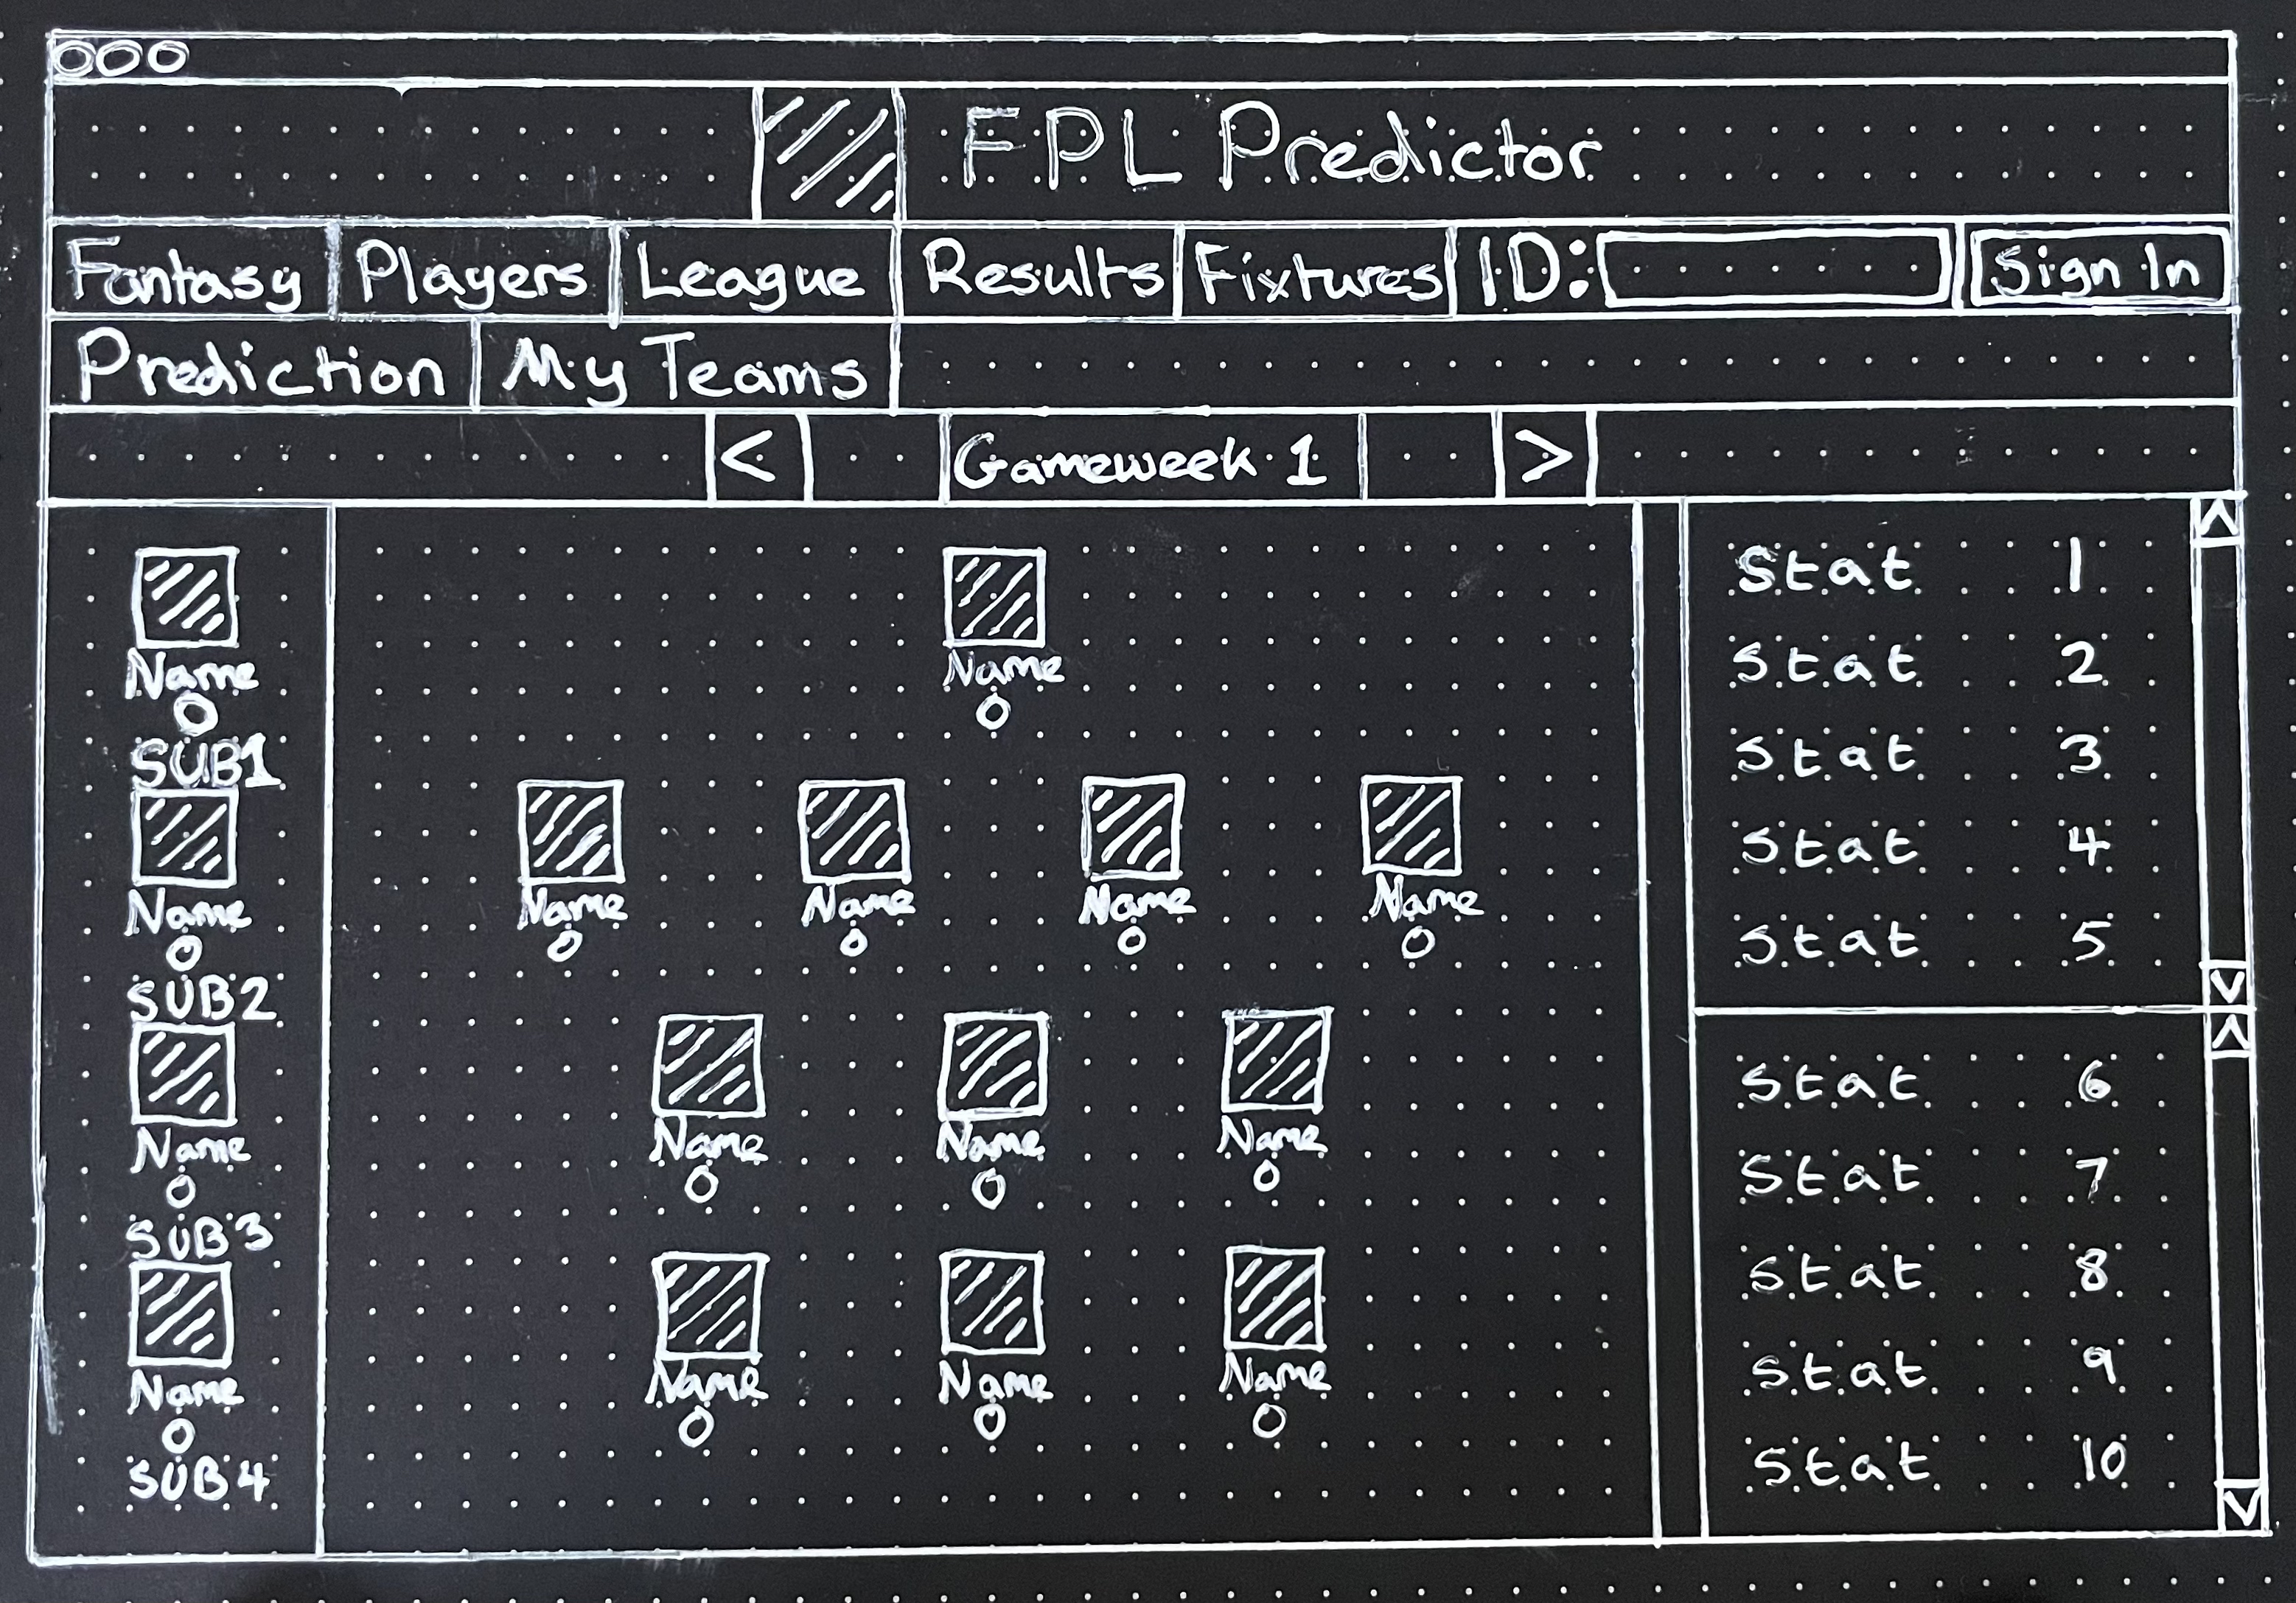
\includegraphics[width=0.75\textwidth]{images/gui/design/wire_frame.jpg}}

\end{image}

The \hyperref[Main page wire-frame]{wire-frame design} above shows exactly how we plan to build the GUI and `Fantasy' tab in our front-end. At the top of the design we can see the title `FPL Predictor' (Fantasy Premier League Predictor) and to the left, a dashed out square indicating the place for a logo. For now, we plan for that to be the Premier League Logo as this is not for commercial use.

Below this we see five rectangles containing the names of our tabs; the Fantasy tab is the tab currently being shown. In the top right we see a text-box followed by a `Sign in' button, which will be where the user enters their FPL manager ID to sign in and access their teams.

Below the main tabs, we see two sub-tabs; `Prediction' and `My Teams'. Both of these tabs will contain similar content, which is shown in the rest of the design, but containing data based on their tab's name; the `Prediction' tab will show predicted teams and `My Teams' will show the user's previous teams.

Teams will be split by each gameweek and will have left and right buttons to switch between the different weeks, as shown in the design. Similarly, the upper half of the stats on the right hand side will also change per gameweek to show the statistics of that current week. However, the lower stats will be overall stats; these will be the same stats showing, no matter whaich gameweek the user is viewing. Moreover, both of these stat tables will have scroll bars in order to view all of the data if there are too many stats to show on one screen.

In the centre of the design we can see eleven dashed out squares which represent players. The squares can be in any valid formation and contain the player image, name and points tally for the gameweek.

On the left hand side of the design, we see four more dashed squares which represent the substitutes, similarly to the other players, the player's image, name and points tally will be shown. Moreover, despite it not being visible in the design, we will also include an indicator as to whether a player is a captain or vice-captain.

Finally, we also plan to have a list view for the teams to give the user multiple ways to view with ease. A similar approach will be adopted when showing the data for the other tabs as they will all require list-like views for what they intend to show.

\section{Java Swing}\label{sec:6.2}

Java Swing is a built-in Java package which can be used to add widgets containing data onto a frame. The main reason why we chose to use this package is it's ability to change it's look and feel depending on the platform it is being used on.

Another reason why I chose to use this package is because of IntelliJ's bulit-in GUI designer. This allows users to create a form containing Swing components in a pane, instead of a frame. Rather than programming a full Swing frame and components from scratch, the Form Designer feature lets users design a basic layout by dragging default widgets into a pane. The layout is naturally split evenly ino columns and rows, for example, if we have two rows and two columns, the pane is split into quarters. Using the `Fill' align options, the component stretches to fill the space it is in. This feature is so useful when designing a program as it enables us to keep a balenced shape and avoid uneccessary spaces.

Java Swing has many other features which make it more than suitable for creating a user interface, such as it's `action listener's. These are features that can be added to a component to listen to any actions made by the user. For example, an action listener may be added to a button to activate a function when the button is clicked. We have used these throughout our program and an example of how this is done is shown below:

\begin{codeblock} \label{Add Action Listener to Button}
  Add Action Listener to Button

  button.addActionListener(e -> \{

  \hspace{\parindent}do something

  \}
\end{codeblock}

As shown in \hyperref[Add Action Listener to Button]{code block 6.2.1}, it is possible to create a function, add it to an action listener, and then add the action listener to a component. It is possible to use many different listeners, such as mouse listeners which track where your device's mouse is on the screen. However, we do not currently have any features which would require these types of listeners, but these could be added in the future. For now, we will stick to using action listeners.

One of the main Swing components we have used in our program is a JTable, which in conjuction with a JScrollPanel, is a very useful component. The purpose of a JTable is to work like any other table by storing data in rows and columns. This is something which we have used throughout all the tabs in the program. In order to store data in a JTable, we make use of the `DefaultTableModel' component, with the parameters being the data and column headers. Furthermore, we can then set the data type of each column, which enables us to use other features such as auto sorting and also the use of renderers. An example of how we create a table model is shown below:

\begin{codeblock} \label{Defining a DefaultTableModel}
  Defining a DefaultTableModel

  DefaultTableModel tableModel = new DefaultTableModel(tableData, tableColumns) \{
    
  \hspace{\parindent}Class<?>[] types = classTypes;

  \hspace{\parindent}@Override

  \hspace{\parindent}public Class<?> getColumnClass(int columnIndex) \{
  
  \hspace{\parindent}\hspace{\parindent}return this.types[columnIndex];
  
  \hspace{\parindent}\}

  \hspace{\parindent}public boolean isCellEditable(int row, int column) \{
  
  \hspace{\parindent}return false;
  
  \hspace{\parindent}\}
  
  \};
\end{codeblock}

The parameters shown in \hyperref[Defining a DefaultTableModel]{code block 6.2.2}; tableData and tableColumns, are of types object array array (Object[][]) and string array (String[]) respectively.

The `tableColumns' variable in \hyperref[Defining a DefaultTableModel]{code block 6.2.2} contains the names of each column header in an array. We take these in as String type as they will never be anything but a label; they are not included in the filtering or sorting of rows and are completely static.

Whereas, the `tableData' variable contains the rows and columns of data that we want to be shown in the table. This data is taken from the respective `.json' files, depending on the table we are filling; this data is taken using the following codeblock:

\begin{codeblock} \label{Creating a DataTable object}
  Creating a DataTable object

  JSONParser parser = new JSONParser();

  try \{

  \hspace{\parindent}JSONArray jsonArray = (JSONArray) parser.parse(new FileReader(fileDir));

  \hspace{\parindent}ArrayList<LinkedHashMap<String, String>> tableValues = new ArrayList<>();

  \hspace{\parindent}for (Object arrObject : jsonArray) \{

  \hspace{\parindent}\hspace{\parindent}JSONObject object = (JSONObject) arrObject;

  \hspace{\parindent}\hspace{\parindent}LinkedHashMap<String, String> row = new LinkedHashMap<>();

  \hspace{\parindent}\hspace{\parindent}for (String columnHeader : columnHeaders) \{

  \hspace{\parindent}\hspace{\parindent}\hspace{\parindent}row.put(columnHeader, String.valueOf(object.get(columnHeader)));

  \hspace{\parindent}\hspace{\parindent}\}

  \hspace{\parindent}\hspace{\parindent}tableValues.add(row);

  \hspace{\parindent}\}

  \hspace{\parindent}return tableValues;

  \} catch (Exception ignored) \{ \}

  return null;
\end{codeblock}

\hyperref[Creating a DataTable object]{Code block 6.2.3} is the code inside the `DataTable' class in our Java program. It's purpose is to extract the data from a `.json' file and store it in a suitable way for the DefaultTableModel to read. We do this by first creating a `JSONParser' object, which is used to read the JSON structure from the file sent as a parameter. We read this data into a `JSONArray' object and split this object into JSONObject objects (containing the data from each row). Then we take each value and pair it with it's corresponding key (column name), putting these rows into a `LinkedHashMap' object and finally returning the object we created. This is the `tableData' variable parsed in \hyperref[Defining a DefaultTableModel]{code block 6.2.2}.

\section{Theme}\label{sec:6.3}

The theme of the GUI will follow a similar theme to the Premier League in terms of the colour scheme. However, there are two themes which can be used throughout the program; light and dark modes.

The light theme is the default theme on start-up and consists of a primarily light colour scheme with white/grey component backgrounds, but with black text. The logo in this theme is purple (matching the same purple colour used in the premier league website).

In order to have a clean product output, we use use the `FlatLaf' library, which is a library which changes the look and feel of a Java Swing interface. The purpose of this look is to give the program a flat look with no shadows or gradients. In our program we use two different FlatLaf themes in `FlatLightLaf' and `FlatDarkLaf', which are FlatLaf light and dark themes respectively. When the program is in dark mode (FlatDarkLaf), our component backgrounds are black/dark grey and our test is white; furthermore, our logo is then set to a green colour (the same green used in the Premier League's colours).

The program's uses the same font throughout each page and component, this being a font called `Quicksand', however different sizes are used depending on the component. The title is set as font size 36, the JTable headers are size 15 and table body is set at 13.

\section{Main Frame}\label{sec:6.4}

The main frame in our product is the one section of the product which will always be shown and is where the user can access each tab. This is the most important part of the interface in terms of visualisation and attraction for this reason. Below is an example of how our main frame will look when it is first opened (for simplicity, we will stick to looking at only the main frame, ignoring the content in the tabs):

\begin{image} \label{Main frame}

  Main frame

  \vspace{0.5cm}

  \centerline{\includegraphics[width=1\textwidth]{images/gui/main/main-frame.png}}

\end{image}

The first functional component in this frame is the light/dark mode button which changes between our themes, described in the \hyperref[sec:6.3]{Theme section}; this component is shown below:

\begin{image} \label{Dark mode button}

  Dark mode button

  \vspace{0.5cm}

  \centerline{\includegraphics[width=0.75\textwidth]{images/gui/theme/dark-mode-button}}

\end{image}

\begin{image} \label{Light mode button}

  Light mode button

  \vspace{0.5cm}

  \centerline{\includegraphics[width=0.75\textwidth]{images/gui/theme/light-mode-button}}

\end{image}

As you can see in images \hyperref[Dark mode button]{6.3.1} and \hyperref[Light mode button]{6.3.2}, the different themes have a very obvious difference and can very easily be switched between. The following shows exactly how we made this possible within a single button:

\begin{codeblock} \label{Light/dark mode JButton}

  Light/dark mode JButton

  colourModeButton.addActionListener(e -> \{

  \hspace{\parindent}if (Objects.equals(colourModeButton.getText(), "Dark Mode")) \{

  \hspace{\parindent}\hspace{\parindent}try \{

  \hspace{\parindent}\hspace{\parindent}\hspace{\parindent}UIManager.setLookAndFeel(new FlatDarculaLaf());

  \hspace{\parindent}\hspace{\parindent}\hspace{\parindent}changeLaF("Light Mode", plLogoGreen);

  \hspace{\parindent}\hspace{\parindent}\} catch (UnsupportedLookAndFeelException ignored) \{\}
  
  \hspace{\parindent}\}
  
  \hspace{\parindent}else if (Objects.equals(colourModeButton.getText(), "Light Mode")) \{
  
  \hspace{\parindent}\hspace{\parindent}try \{
  
  \hspace{\parindent}\hspace{\parindent}\hspace{\parindent}UIManager.setLookAndFeel(new FlatLightLaf());
  
  \hspace{\parindent}\hspace{\parindent}\hspace{\parindent}changeLaF("Dark Mode", plLogoPurple);
  
  \hspace{\parindent}\hspace{\parindent}\} catch (UnsupportedLookAndFeelException ignored) \{\}
  
  \hspace{\parindent}\}
  
  \});

\end{codeblock}

Firstly we must check which theme we wish to chenge to (if in dark mode, we change to light mode and vice-versa) by getting the text on the button. We then compare set the look and feel in the UIManager using `.setLookAndFeel' and run our changeLaF method with the parameters based on whichever theme we wish to switch to. This is added as a listener to a button so that whenever the button is pressed by the user, the action commences.

Below we see our `changeLaF' method which changes the other components in our program, based on whether we are in the light or dark theme:

\begin{codeblock} \label{changeLaF method}

  changeLaF method

  public void changeLaF(String text, Icon logo) \{
  
  \hspace{\parindent}colourModeButton.setText(text);
  
  \hspace{\parindent}FlatLaf.updateUI();
  
  \hspace{\parindent}logoLabel.setIcon(logo);
  
  \}

\end{codeblock}

The \hyperref[changeLaF method]{changeLaF method} parses two parameters; a string variable containing the new button text and a string variable containing a link to the new logo image. This method sets the text of the Light/Dark JButton, sets the icon of the logo label to the image in the path provided and updates the interface's look and feel to match the chosen mode.

The other functional component we see in the \hyperref[Main frame]{main frame} is a JTabbedPane. This is a component which allows us to have multiple pages which can be accessed by selecting each tab. These are easily programmed using the Swing Designer Form.

\section{Fantasy Tab}\label{sec:8.5}

The `Fantasy' tab in our program contains two sub-tabs; `Predicted Teams' and `My Teams' tabs. Each of these sub-tabs also contain two sub-sub-tabs; `Pitch View' and `List View'. The design of the sub-tabs `Predicted Teams' and `My Teams' are exactly the same design, however one shows our team predictions and the other shows a manager's past teams (if a Manager ID has been inputted). Below we see our `Fantasy' tab open in the Swing Designer Form:

\begin{image} \label{Fantasy tab in the Swing Designer Form}

  Fantasy tab in the Swing Designer Form

  \vspace{0.5cm}

  \centerline{\includegraphics[width=0.6\textwidth]{images/gui/fantasy-tab/fantasy-tab-swing-designer}}

\end{image}

As we can see in the \hyperref[Fantasy tab in the Swing Designer Form]{above image}, most of the designing for this part of the program is hard-coded through the Swing Designer Form using various components. We make use of the spacers in order to evenly spread our components and have a clear idea of how the program will look visually. Most of the labels and other forms of text have been created through the form; however, many of the components with functionality have to be created or modified within a Java script itself. An example output of this tab is shown below:

\begin{image} \label{Fantasy tab}

  Fantasy tab

  \vspace{0.5cm}

  \centerline{\includegraphics[width=1\textwidth]{images/gui/fantasy-tab/output.png}}

\end{image}

The most important part of this tab, like any other, is the displaying of our information. For each player we have a square-shaped JFrame containing four blank labels; these labels are where we show our data. This is shown below:

\begin{image} \label{Player in the Swing Designer Form}

  Player in the Swing Designer Form

  \vspace{0.5cm}

  \centerline{\includegraphics[width=0.25\textwidth]{images/gui/fantasy-tab/player-form.png}}

\end{image}

Referring to the \hyperref[Player in the Swing Designer Form]{player design} above, the placement of each piece of data follows suit with our \hyperref[Main page wire-frame]{wire-frame design}; we have the player's image in the top left, captaincy icon in the top right, name in the middle and point count at the bottom as shownin our output below:

\begin{image} \label{Player in program output}

  Player in program output

  \vspace{0.5cm}

  \centerline{\includegraphics[width=0.25\textwidth]{images/gui/fantasy-tab/player.png}}

\end{image}

Furthermore, we have also used this player JFrame in a more complex way in order to shown the correct formation of the team. As stated in the \hyperref[managing your squad rules]{rules}, the user may use a number of formations. For this reason, we must make use of Swing's `CardLayout' type in the `Layout Manager'. This allows us to design multiple `cards' (layouts) and choose which card to show at any time. For example, when a formation with three defenders is being used, we can select our card which has 3 players; if we have four defenders in the formation, we select our four-player card, etc. We split our design up into positions in order to use the least amount of cards necessary, which leaves us with the following:

\begin{itemize}
  \item Goalkeeper
  \begin{itemize}
    \item 1 player card
  \end{itemize}
  \item Defenders
  \begin{itemize}
    \item 3 player card
    \item 4 player card
    \item 5 player card
  \end{itemize}
  \item Midfielders
  \begin{itemize}
    \item 2 player card
    \item 3 player card
    \item 4 player card
    \item 5 player card
  \end{itemize}
  \item Forwards
  \begin{itemize}
    \item 1 player card
    \item 2 player card
    \item 3 player card
  \end{itemize}
\end{itemize}

We do not need to make any layout changes to our goalkeeper as there can only ever be one goalkeeper at a time; therefore, we can leave our goalkeeper JPanel in the default layout. For the other positions, it is necessary to use the `CardLayout' feature, so we create and assign the necessary cards shown above; this is done using the following code:

\begin{codeblock} \label{Create cards}
  Create cards

  LinkedHashMap<JPanel, String[]> myTeamCards = createCards(new String[] \{
  
  \hspace{\parindent}"myDEF3Card", "myDEF4Card", "myDEF5Card",
  
  \hspace{\parindent}"myMID2Card", "myMID3Card", "myMID4Card", "myMID5Card",
  
  \hspace{\parindent}"myFWD1Card", "myFWD2Card", "myFWD3Card"

\}, new JPanel[] \{myDEFPanel, myMIDPanel, myFWDPanel\});

\vspace{0.5cm}

  public LinkedHashMap<JPanel, String[]> createCards(String[] cardNames, JPanel[] panelNames) \{

  \hspace{\parindent}LinkedHashMap<JPanel, String[]> cards = new LinkedHashMap<>();

  \hspace{\parindent}int cardCounter = 0;

  \hspace{\parindent}int panelCounter = 0;
        
  \hspace{\parindent}for (int amount : new int[] {3, 4, 3}) \{
            
  \hspace{\parindent}\hspace{\parindent}String[] cardArray = new String[amount];
            
  \hspace{\parindent}\hspace{\parindent}for (int i = 0; i < amount; i++) \{
                
  \hspace{\parindent}\hspace{\parindent}\hspace{\parindent}cardArray[i] = cardNames[cardCounter];
                
  \hspace{\parindent}\hspace{\parindent}\hspace{\parindent}cardCounter +=1;
            
  \hspace{\parindent}\hspace{\parindent}\}
            
  \hspace{\parindent}\hspace{\parindent}cards.put(panelNames[panelCounter], cardArray);
            
  \hspace{\parindent}\hspace{\parindent}panelCounter += 1;
        
  \hspace{\parindent}\}
        
  \hspace{\parindent}return cards;
    
  \}

\end{codeblock}

\hyperref[Create cards]{Code block 8.5.4} contains two methods, which together create and assign our JPanels to our cards' LinkedHashMap. The first class is just one of the instances where we create and assign our cards as we do this multiple times. The best way to store these cards is in a LinkedHashMap as we found that when working out the correct formation, it works well with our algorithm. In our second method, we use a nested for loop and two counters to assign panels to positions in our `cards' variable.

Now that we have created all of the necessary cards per position, the card selection process begins, based on the formation of the team we are showing. We use a simple algorithm to work out which formation we are using, as shown below:

\begin{codeblock} \label{Calculate formation}

  Calculate formation

  int[] formation = \{1, 0, 0, 0\};
  
  for (HashMap<String, String> player : tableList) \{
  
  \hspace{\parindent}if (Integer.parseInt(player.get("position")) <= 11) \{
  
  \hspace{\parindent}\hspace{\parindent}String position = player.get("position\_name");
  
  \hspace{\parindent}\hspace{\parindent}switch (position) \{
  
  \hspace{\parindent}\hspace{\parindent}\hspace{\parindent}case "DEF":

  \hspace{\parindent}\hspace{\parindent}\hspace{\parindent}\hspace{\parindent}formation[1] += 1;

  \hspace{\parindent}\hspace{\parindent}\hspace{\parindent}\hspace{\parindent}break;

  \hspace{\parindent}\hspace{\parindent}\hspace{\parindent}case "MID":

  \hspace{\parindent}\hspace{\parindent}\hspace{\parindent}\hspace{\parindent}formation[2] += 1;

  \hspace{\parindent}\hspace{\parindent}\hspace{\parindent}\hspace{\parindent}break;
  
  \hspace{\parindent}\hspace{\parindent}\hspace{\parindent}case "FWD":

  \hspace{\parindent}\hspace{\parindent}\hspace{\parindent}\hspace{\parindent}formation[3] += 1;

  \hspace{\parindent}\hspace{\parindent}\hspace{\parindent}\hspace{\parindent}break;

  \hspace{\parindent}\hspace{\parindent}\}

  \hspace{\parindent}\}

  \}

\end{codeblock}

We store our formation in an array with the goalkeeper already entered in the first position being `1', We then go through the first 11 players in our team and get their positions. We then use a switch statement to compare each player's position to our options and add to our array for each position. This leaves us with an array containing the amount of players in each position, stored in the variable `formation'.

Following this, we then call our `setCard()' method and send all of the card panels and our formation array as parameters; this method is shown below:

\begin{codeblock} \label{setCard method}

  setCard() method

  int i = 1;
  
  int[] amount = new int[] \{3, 2, 1\};
  
  for (JPanel panel : panels.keySet()) \{
  
  \hspace{\parindent}CardLayout card = (CardLayout) panel.getLayout();
  
  \hspace{\parindent}card.show(panel, panels.get(panel)[formation[i]-amount[i-1]]);
  
  \hspace{\parindent}i += 1;
  
  \}

\end{codeblock}

The \hyperref[setCard method]{setCard() method} simply uses an array containing the differences between the two parameters, then runs through the formation array and choses the correct card to be displayed per position.

Finally, we pull the player data from our arrayList and put the correct data in the correct labels, including the substitutes who have their own display section on the left-hand side. The result of this is shown below:

\begin{image} \label{Team in pitch view}

  Team in pitch view

  \vspace{0.5cm}

  \centerline{\includegraphics[width=1\textwidth]{images/gui/fantasy-tab/team-pitch-view.png}}

\end{image}

The `List View' tab contains a JTable component which shows the players in the displayed team in a list, in slightly more detail. We create a table in the Swing Form, but add the data using the methods shown in code blocks \hyperref[Defining a DefaultTableModel]{8.2.2} and \hyperref[Creating a DataTable object]{6.2.3}.

This is an example of how our tab looks once we have inserted the data:

\begin{image} \label{Team in pitch view}

  Team in pitch view

  \vspace{0.5cm}

  \centerline{\includegraphics[width=1\textwidth]{images/gui/fantasy-tab/team-list-view.png}}

\end{image}

Not only is this table visually appleasing, it is also interactive. As we have set the data types of each of the columns in this table, we can sort each column by pressing the header. The sort procedure used depands on the columns data type; for example, the first unnamed column and our points columns are sorted based on the total points and can be switch from ascending to descending with a single click. The other columns are sorted alphabetically, and can also wbe switched from ascending to descending or vice-versa at any time.

An example of our table being sorted by the `Points' column in descending order is shown below:

\begin{image} \label{Team sorted by points}

  Team sorted by points

  \vspace{0.5cm}

  \centerline{\includegraphics[width=1\textwidth]{images/gui/fantasy-tab/team-list-view-sorted.png}}

\end{image}

Another feature of our tables is that we can change the column order. This is useful when we are focusing on just a few of the shown columns. If the user drags the column header, the column will move and snap into place upon release.

If a user wanted to make a comparison between between the points per player, the two most important columns are the player's `Name' and `Points'. However, these columns are not close together, which is an inconvenience. An example of this feature being used to solve this inconvenience is shown below:

\begin{image} \label{Moving columns in our table}

  Moving columns in our table

  \vspace{0.5cm}

  \centerline{\includegraphics[width=1\textwidth]{images/gui/fantasy-tab/team-list-view-columns-moved.png}}

\end{image}

There are two other types of components in this tab which are also tables; they show the manager's stats and also the gameweek stats. These are not a part of the pitch or list view and are shown no matter which view we are showing as they are a part of the main sub-tabs. The manager stats table shows data about the manager or prediction overall and has the same data shown, no matter which gameweek is being viewed. However, the Gameweek Stats table updates it's data depending on which gameweek we are viewing as the data is specifically about that gameweek. An example of how the tables look is shown below:

\begin{image} \label{Stats tables}

  Stats tables

  \vspace{0.5cm}

  \centerline{\includegraphics[width=0.3\textwidth]{images/gui/fantasy-tab/stats-tables.png}}

\end{image}

Our stats tables both have scroll bars for when all of the data is not visible. Sorting is not possible on these table's columns, as the data is of dfferent types, making it completely unneccessary.

In order to change which gameweek is being viewed, we have two JButton components, which work as simple left/right buttons. Pressing the left button changes to the week before; pressing the right button changes to the following week. Obviously the buttons are disabled if there is no week before or after the current gameweek being shown. Below, our gameweek label and buttons are shown:

\begin{image} \label{Gameweek label and buttons}

  Gameweek label and buttons

  \vspace{0.5cm}

  \centerline{\includegraphics[width=1\textwidth]{images/gui/fantasy-tab/Gameweek-label-and-buttons.png}}

\end{image}

For us to know how many gameweeks we have data for, we take the data from our `list-of-gameweeks.json' file and store it in an array. We then use the buttons to activate a counter variable which moves between positions in the array. Whenever a button is refreshed, we refresh the necessary components, for example, the gameweek label is changed, we get new table data for the corresponding week and we update the pitch and list view graphics.

\vspace{0.5cm}

The final components we have in our fantasy tab are the manager ID text-box and sign in button, which work in-conjuction with each other, in order for the user to see their previous fantasy football teams. These components are shown below:

\begin{image} \label{Sign-in}

  Sign-in

  \vspace{0.5cm}

  \centerline{\includegraphics[width=1\textwidth]{images/gui/fantasy-tab/sign-in.png}}

\end{image}

\begin{image} \label{Signed-in}

  Signed-in

  \vspace{0.5cm}

  \centerline{\includegraphics[width=1\textwidth]{images/gui/fantasy-tab/signed-in.png}}

\end{image}

One of the API requests we were using required credentials to get the current team the user has, but taking the user's username and password for their account was decided against due to security reasons. Moreover there is no real benefit of seeing the current chosen team of a player, as it is not possible to officially make changes to a team using our application.

The manager ID text-box has the purpose of taking in the user's inputted text, completing validation check to make sure it is a valid ID and calling the Python script to collect the data. Below is the code which completes the validation check of the ID:

\begin{codeblock} \label{Check ID validity}

  Check ID validity

  try \{
            
  \hspace{\parindent}Integer.parseInt(managerId);
        
  \} catch (NumberFormatException notInteger) \{
            
  \hspace{\parindent}return false;
        
  \}
        
  return getAPIResponse("https://fantasy.premierleague.com/api/entry/" + managerId + "/");

\end{codeblock}

The first validation check that is made is to make sure that the inputted data is an integer as a Manager ID cannoy contain any non-integer characters. If the text is vaid, we can check there is a response from the API which can be done as follows:

\begin{codeblock} \label{getAPIResponse method}

  getAPIResponse() method~\cite{HTTP response code in Java}

  try \{

  \hspace{\parindent}URL url = new URL(urlStr);

  \hspace{\parindent}HttpURLConnection connection = (HttpURLConnection) url.openConnection();

  \hspace{\parindent}connection.setRequestMethod("GET");

  \hspace{\parindent}connection.connect();

  \hspace{\parindent}connection.getPermission();

  \hspace{\parindent}return connection.getResponseCode() != 404;

  \} catch (Exception ignored) \{

  \hspace{\parindent}return false;

  \}

\end{codeblock}

Using the \hyperref[getAPIResponse method]{getAPIResponse() method} we either can't connect to the API if the manager ID is not valid, or if there is an issue retreiving the data, we can receieve a respose code of `404'. Both of these outcomes will result in us not having data to show, so we ensure that we recieve a valid response code before we attempt to pull the data from the API through Python. If we do not manager to get any data for the inputted manager ID for any reason, the user sees the following:

\begin{image} \label{Incorrect manager id}

  Incorrect manager ID

  \vspace{0.5cm}

  \centerline{\includegraphics[width=1\textwidth]{images/gui/fantasy-tab/incorrect-manager-id.png}}

\end{image}

There is a brief time-delay when using the sign-in function which is not ideal, which hopefully can be shortened in the future. However, to not confuse the user, we make the tab unclickable, until the sign-in process is finished and there is data to be viewed. The following shows what this looks like:

\begin{image} \label{Unclickable tab}

  Unclickable tab

  \vspace{0.5cm}

  \centerline{\includegraphics[width=0.5\textwidth]{images/gui/fantasy-tab/unclickable-tab.png}}

\end{image}

Moreover, similarly to the Predicted Teams tab, we have both a pitch and list view tab which contains the exact same functioning components.

\section{Players Tab}\label{sec:6.6}

The `Players' tab contains a database-like table, useful for searching fantasy stats about players. We create this table using a JTable components and enter our data using the methods shown in code blocks \hyperref[Defining a DefaultTableModel]{6.2.2} and \hyperref[Creating a DataTable object]{8.2.3}. Our table headers are of font size 15 and body size 13 and all of the cells are centered horizontally using our custom table renderers. The order of the columns in this table can be modified and the rows can be filtered by a particular column. Below is how our players tab looks in both our light and dark modes:

\begin{image} \label{Players tab in light mode}

  Players tab in light mode

  \vspace{0.5cm}

  \centerline{\includegraphics[width=1\textwidth]{images/gui/players-tab/light.png}}

\end{image}

\begin{image} \label{Players tab in dark mode}

  Players tab in dark mode

  \vspace{0.5cm}

  \centerline{\includegraphics[width=1\textwidth]{images/gui/players-tab/dark.png}}

\end{image}

\section{League Table Tab}\label{sec:6.7}

Our `League table' tab shows a live league table for the Premier League, as you would expect. We use a JTable component to do create the table and enter our data using the methods shown in code blocks \hyperref[Defining a DefaultTableModel]{6.2.2} and \hyperref[Creating a DataTable object]{6.2.3}. Our table headers and body are of sizes 15 and 13 respectively and all of the cells are centered horizontally using our custom table renderers. The order of the columns in this table can be modified to allow team comparisons to be made easier, however, no filters can be applied to the data as the purpose of this table is to provide the user with an official order, based on the official tabling rules of the Premier League. The table is inside a JScrollPanel, which allows us to scroll throught the table if not all of the data is visible. Below is how our live league table looks in both our light and dark modes:

\begin{image} \label{League table tab in light mode}

  League table tab in light mode

  \vspace{0.5cm}

  \centerline{\includegraphics[width=1\textwidth]{images/gui/league-table-tab/light.png}}

\end{image}

\begin{image} \label{League table tab in dark mode}

  League table tab in dark mode

  \vspace{0.5cm}

  \centerline{\includegraphics[width=1\textwidth]{images/gui/league-table-tab/dark.png}}

\end{image}

\section{Results Tab}\label{sec:8.8}

The Results tab shows the latest results of the Premier League in a JTable component. The default order of the table is to show from the most recent to oldest results; this order cannot be changed as no filters can be applied to the columns. In the future, it would be ideal to have a drop-down to allow the user to select a team, only the matches of that team would then be shown.

The column order in this table can be modified to allow users to choose how they view the data. However, this does uncover a design flaw as the user can switch `Home Team' and `Away Team' columns, as well as the badge columns, in order to switch all of the results. I do not see why a user would do this, unless as a mistake. The only way to fix this issue would be to have the team names, badges and scores in one column, but this would remove almost all of the column order modification options and defeat the point of the whole feature. Furthermore, the font style and sizing follows suit with the other tables in the program.

\begin{image} \label{Results tab in light mode}

  Results tab in light mode

  \vspace{0.5cm}

  \centerline{\includegraphics[width=1\textwidth]{images/gui/results-tab/light.png}}

\end{image}

\begin{image} \label{Results tab in dark mode}

  Results tab in dark mode

  \vspace{0.5cm}

  \centerline{\includegraphics[width=1\textwidth]{images/gui/results-tab/dark.png}}

\end{image}

\section{Fixtures Tab}\label{sec:6.9}

This tab is extremely similar to the `Results' tab in terms of shown data, it's types and the component functionality. Once again, we use a JTable to store our data, which is retreived and displayed using code blocks \hyperref[Defining a DefaultTableModel]{6.2.2} and \hyperref[Creating a DataTable object]{8.2.3}. In terms of table functionality, we can change our column order through simply dragging the column's header or body to the desired location. The same renderers are applied to the table, which horizontally centers our text and sets our font to `Quicksand' and font sizes to 15 and 13.

\begin{image} \label{Fixtures tab in light mode}

  Fixtures tab in light mode

  \vspace{0.5cm}

  \centerline{\includegraphics[width=1\textwidth]{images/gui/fixtures-tab/light.png}}

\end{image}

\begin{image} \label{Fixtures tab in dark mode}

  Fixtures tab in dark mode

  \vspace{0.5cm}

  \centerline{\includegraphics[width=1\textwidth]{images/gui/fixtures-tab/dark.png}}

\end{image}

The above images once again shows the difficulty of predicting the Premier League, when game cancellations, illnesses and other issues arise from non-football related problems such as Covid-19. 

\chapter{Application}\label{ch:7}

Our application's prediction method and data handling is written in Python and the interface is in Java; this allows us to have two different ways to run our program. When running our program in Python, we get a command-line output of our prediction, compared to a fully working application when running our java program.

\section{Libraries and Imports}\label{sec:7.1}

Before the application is run, there are many libraries used by both our Python and Java scripts which must be downloaded. Without these, the program will either be very limited in some coases, or more likely unable to be run.

Please ensure that all libraries are installed before attempting to run the program.

Below is the list of libraries and imports we use (of which all are the latest versions as of when this report is dated):

\begin{itemize}
  \item \href{https://pypi.org/project/requests/}{requests}
  \item \href{https://docs.python.org/3/library/os.html}{os} (built-in)
  \item \href{https://pandas.pydata.org/docs/getting_started/install.html}{pandas}
  \item \href{https://pypi.org/project/Unidecode/}{Unidecode}
  \item \href{https://pypi.org/project/numpy/}{numpy}
  \item \href{https://pypi.org/project/pytest-shutil/}{shutil}
  \item \href{https://pypi.org/project/scikit-learn/}{sklearn}
  \item \href{https://pypi.org/project/PuLP/}{PuLP}
  \item \href{https://www.json.org/json-en.html}{JSON} (built-in)
  \item \href{https://docs.oracle.com/javase/7/docs/api/java/io/package-summary.html}{java.io} (built-in)
  \item \href{https://mkyong.com/java/json-simple-example-read-and-write-json/}{JSON.simple}
  \item \href{https://docs.oracle.com/javase/8/docs/api/java/util/package-summary.html}{java.util} (built-in)
  \item \href{https://www.formdev.com/flatlaf/}{FlatLaf}
  \item \href{https://docs.oracle.com/javase/7/docs/api/java/net/package-summary.html}{java.net} (built-in)
  \item \href{https://docs.oracle.com/javase/8/docs/api/javax/swing/package-summary.html}{javax.swing} (built-in)
  \item \href{https://docs.oracle.com/javase/7/docs/api/java/awt/package-summary.html}{java.awt} (built-in)
  \item \href{https://docs.oracle.com/javase/8/docs/api/javax/imageio/ImageIO.html}{javax.imageio}
\end{itemize}

\section{Options}\label{sec:7.2}

Before running the program, we have the option of whether to use the live fixture data for our prediction or whether to use the data from the GitLab repository (currently week 30). We can set this by going to the Python file  at `/python/data.py' and setting the `live = True' to use live data or `live = False' for non-live data.

Before the decision is made, lets review the positives and negatives of each:

Live data:
\begin{itemize}
  \item Live team prediction from gameweek 1 to next week's gameweek
  \item Takes around two to two and a half minutes to run the program (depending on your machine)
\end{itemize}

Non-live data:
\begin{itemize}
  \item Team prediction from gameweek 1 to gameweek 30 (or later if the data is replaced with later commits from the GitHub Repository)
  \item Takes around 15 to 25 seconds to run the program (depending on your machine)
\end{itemize}

\section{Running Python}\label{sec:7.3}

The program can be run from python file `/python/main.py', which produces a summary of our solved linear programming model and an output of our initial team. We then see how many points our initial team would get over the course of the season with no transfers. We are then shown the transfers made for each week, how many points we get and finally a points total over the season so far. It takes around two minutes to run with live data and 15 seconds with non-live data.

\section{Running Java}\label{sec:7.4}

When we run our java program `src/src/main/java/Main.java', we are shown an application consisting of tabs; `Fantasy', `Players', `League Table', `Results' and `Fixtures'. When we run this Java file, all of the Python scripts we use are run also. It takes around two and a half minutes to run with live data and 25 seconds with non-live data. It then takes a further 40 seconds more to sign in with a manager ID.

\chapter{Conclusion}\label{ch:concl}

The overall application tool we have produced has a very simple and appealing interface, with a decent amount of functionality, enough for it's purpose. Each section of the program could have been improved if given more time, but a valient effort was made across the board to have a fully-functioning program. Creating an application for a game made by one of the largest companies in a sector is so difficult, as these companies know how important it is to gate-keep certain parts of their business in order to stay at the top.  For example, actually being able to make changes to our team in a fully interactive way would have been a very nice feature to implement. However, it is not possible for any third-party application to do so.

All of the tabs in our application are informative, with the most useful being the fantasy tab. Not only did we manage to make a prediction for the entire season of football so far, we also found a way to show our prediction in a very visually appealing way.

With this being such a large project to take on, it is understandable that we did not manage to create a perfect prediction model, neither did we manage to create a flawless application which could compete with the likes of the Premier League. This was a chance to learn and practice new skills from both a mathematical prediction and a graphical design viewpoint. The most important aspect we can take from this project is that it was built correctly, meaning that improvements can be made with ease.


\begin{thebibliography}{999}

  \bibitem{Premier League Data Capture}
  Premier League.
  \newblock `Statistics Explained'.
  \newblock {\em Premier League, https://www.premierleague.com/stats/clarification. [Last accessed: 16 November 2021]}

  \bibitem{API Definition}
  IBM Cloud Education.
  \newblock `Application Programming Interface (API)'.
  \newblock {\em IMB, https://www.ibm.com/cloud/learn/api. [Last accessed: 16 November 2021]}

  \bibitem{Requests}
  Unknown.
  \newblock `Requests: HTTP for Humans'.
  \newblock {\em Requests http for humans, https://docs.python-requests.org/en/latest/. [Last accessed: 15 November 2021]}
  
  \bibitem{Preprocessing definition}
  Unknown.
  \newblock `Data Preprocessing'.
  \newblock {\em techopedia, 11 July 2021, https://www.techopedia.com/definition/14650/data-preprocessing. [Last accessed: 15 November 2021]}

  \bibitem{Preprocessing techniques}
  Rajaratne, Maneesha.
  \newblock `Data Pre Processing Techniques You Should Know'.
  \newblock {\em towards data science, 2 December 2018, https://towardsdatascience.com/data-pre-processing-techniques-you-should-know-8954662716d6.}
  
  \bibitem{API Endpoints}
  Timothy, Frenzel.
  \newblock `Fantasy Premier League API Endpoints: A Detailed Guide'.
  \newblock {\em Medium, 8 October 2020, https://medium.com/@frenzelts/fantasy-premier-league-api-endpoints-a-detailed-guide-acbd5598eb19.}

  \bibitem{HTTP response code in Java}
  Rob Hruska and Ravi.
  \newblock `How to get HTTP response code for a URL in Java?'.
  \newblock {\em Stack overflow, 4 February 2018, https://stackoverflow.com/questions/6467848/how-to-get-http-response-code-for-a-url-in-java.}

  \bibitem{Check for NaN}
  Unknown.
  \newblock `Check for NaN in Pandas DataFrame (examples included)'.
  \newblock {\em Data to Fish, 10 September 2021, https://datatofish.com/check-nan-pandas-dataframe/.}

  \bibitem{pandas map function}
  Unknown.
  \newblock `pandas.Series.map'.
  \newblock {\em Pandas, https://pandas.pydata.org/docs/reference/api/pandas.Series.map.html.}

  \bibitem{unidecode}
  Unknown.
  \newblock `Python unidecode.unidecode() Examples'.
  \newblock {\em Unidecode, https://www.programcreek.com/python/example/94318/unidecode.unidecode.}

  \bibitem{kaggle project}
  Gavin Ng.
  \newblock `FPL-prediction-and-selection'.
  \newblock {\em Kaggle, https://www.kaggle.com/code/gavinjpng/fpl-prediction-and-selection/notebook.}

  \bibitem{PuLP}
  Unknown.
  \newblock `Optimization with PuLP'.
  \newblock {\em PuLP, https://coin-or.github.io/pulp/.}

  \bibitem{lpProblem}
  Unknown.
  \newblock `The lpProblem Class'.
  \newblock {\em PuLP, https://www.coin-or.org/PuLP/pulp.html\#pulp.LpProblem.}

  \bibitem{skikit-learn}
  Unknown.
  \newblock `Machine Learning in Python'.
  \newblock {\em skikit-learn, https://scikit-learn.org/stable/.}

\end{thebibliography}

\end{document}